%!TEX root = modelguide.tex

\chapter{Mechanical Models II}
\label{MechModelsII:sec}

This section provides additional material on building basic
multibody-type mechanical models.

\section{Simulation control properties}

Both \javaclass[artisynth.core.workspace]{RootModel} and
\javaclass[artisynth.core.mechmodels]{MechModel} contain properties
that control the simulation behavior. One of the most important of
these is {\tt maxStepSize}. By default, simulation proceeds using the
{\tt maxStepSize} value defined for the root model. A {\tt MechModel}
(or any other type of {\tt Model}) contained in the root model's {\tt
models} list may also request a smaller step size by specifying a
smaller value for its own {\tt maxStepSize} property.  For all models,
the {\tt maxStepSize} may be set and queried using
%
\begin{lstlisting}[]
  void setMaxStepSize (double maxh);
  double getMaxStepSize();
\end{lstlisting}
%

Another important simulation property is {\tt integrator} in {\tt
MechModel}, which determines the type of integrator used for the
physics simulation. The value type of this property is the enumerated
type {\tt MechSystemSolver.Integrator}, for which the following values
are currently defined:

\begin{description}

\item[ForwardEuler]\mbox{}

First order forward Euler integrator. Unstable for stiff systems.

\item[SymplecticEuler]\mbox{}

First order symplectic Euler integrator, more energy conserving
that forward Euler. Unstable for stiff systems.

\item[RungeKutta4]\mbox{}

Fourth order Runge-Kutta integrator, quite accurate but also unstable
for stiff systems.

\item[ConstrainedBackwardEuler]\mbox{}

First order backward order integrator. Generally stable for stiff systems.

\item[Trapezoidal]\mbox{}

Second order trapezoidal integrator. Generally stable for stiff
systems, but slightly less so than {\tt ConstrainedBackwardEuler}.

\end{description}

The term ``Unstable for stiff systems'' means that the integrator is
likely to go unstable in the presence of ``stiff'' systems, which
typically include systems containing finite element models, unless the
simulation step size is set to an extremely small value.  The default
value for {\tt integrator} is {\tt ConstrainedBackwardEuler}.

\begin{sideblock}
Stiff systems tend to arise in models containing interconnected
deformable elements, for which the step size should not exceed the
propagation time across the smallest element, an effect known as the
Courant-Friedrichs-Lewy (CFL) condition. Larger stiffness and damping
values decrease the propagation time and hence the allowable step
size.
\end{sideblock}

Another {\tt MechModel} simulation property is {\tt stabilization},
which controls the stabilization method used to correct drift from
position constraints and correct interpenetrations due to collisions.
The value type of this property value is the enumerated type {\tt
MechSystemSolver.PosStabilization}, which presently has two values:

\begin{description}

\item[GlobalMass]\mbox{}

Uses only a diagonal mass matrix for the MLCP that is solved to
determine the position corrections. This is the default method.

\item[GlobalStiffness]\mbox{}

Uses a stiffness-corrected mass matrix for the MLCP that is solved to
determine the position corrections. Slower than {\tt GlobalMass}, but
more likely to produce stable results, particularly for
problems involving FEM collisions.

\end{description}

\section{Units}
\label{sec:mechii:units}

ArtiSynth is primarily ``unitless'', in the sense that it does not
define default units for the fundamental physical quantities of time,
length, and mass. Although time is
generally understood to be in seconds, and often declared as such in
method arguments and return values, there is no hard requirement that
it be interpreted as seconds. There are no assumptions at all
regarding length and mass. Some components may have default parameter
values that reflect a particular choice of units, such as {\tt
MechModel}'s default gravity value of $(0, 0, -9.8)^T$, which is
associated with the MKS system, but these values can always be
overridden by the application.

Nevertheless, it is important, and up to the application developer to
ensure, that units be {\it consistent}. For example, if one decides to
switch length units from meters to centimeters (a common choice),
then all units involving length will have to be scaled appropriately.
For example, density, whose fundamental units are $m/d^3$, where $m$ is mass and
$d$ is distance, needs to be scaled by $1/100^3$, or $0.000001$, when
converting from meters to centimeters.

Table \ref{Units:tab} lists a number of common physical quantities
used in ArtiSynth, along with their associated fundamental units.

\begin{table}
\begin{center}
\begin{tabular}{|lll|}
\hline
unit & fundamental units & \\
\hline
time                    & $t$ & \\
distance                & $d$ & \\
mass                    & $m$ & \\
velocity                & $d/t$ & \\
acceleration            & $d/t^2$ & \\
force                   & $m d/t^2$ & \\
work/energy             & $m d^2/t^2$& \\
torque                  & $m d^2/t^2$ & same as energy (somewhat counter intuitive)\\
angular velocity        & $1/t$ & \\
angular acceleration    & $1/t^2$ & \\
rotational inertia      & $m d^2$ & \\
pressure                & $m/(d t^2)$ & \\
Young's modulus         & $m/(d t^2)$ & \\
Poisson's ratio         & 1 & no units; it is a ratio \\
density                 & $m/d^3$ & \\
linear stiffness        & $m/t^2$ & \\
linear damping          & $m/t$ & \\
rotary stiffness        & $m d^2/t^2$ & same as torque \\
rotary damping          & $m d^2/t$ & \\
mass damping            & $1/t$ & used in FemModel \\
stiffness damping       & $t$ & used in FemModel \\
\hline
\end{tabular}
\end{center}
\caption{Physical quantities and their representation in terms of the
fundamental units of mass ($m$), distance ($d$), and time ($t$).}
\label{Units:tab}
\end{table}

\subsection{Scaling units}

For convenience, many ArtiSynth components, including {\tt MechModel},
implement the interface
\javaclass[artisynth.core.util]{ScalableUnits}, which
provides the following methods for scaling mass and distance units:
%
\begin{lstlisting}[]
  scaleDistance (s);    // scale distance units by s
  scaleMass (s);        // scale mass units by s
\end{lstlisting}
%
A call to one of these methods should cause all physical quantities
within the component (and its descendants) to be
scaled as required by the fundamental unit relationships
as shown in Table \ref{Units:tab}.

Converting a {\tt MechModel} from meters to centimeters can therefore be
easily done by calling 
%
\begin{lstlisting}[]
   mech.scaleDistance (100);
\end{lstlisting}
%
As an example, adding the following code to the end of the {\tt build()}
method in {\tt RigidBodySpring} (Section \ref{RigidBodySpringExample:sec})
%
\begin{lstlisting}[]
   System.out.println ("length=" + spring.getLength());
   System.out.println ("density=" + box.getDensity());
   System.out.println ("gravity=" + mech.getGravity());
   mech.scaleDistance (100);
   System.out.println ("");
   System.out.println ("scaled length=" + spring.getLength());
   System.out.println ("scaled density=" + box.getDensity());
   System.out.println ("scaled gravity=" + mech.getGravity());
\end{lstlisting}
%
will scale the distance units by 100 and print the values of various
quantities before and after scaling. The resulting output is:
%
\begin{lstlisting}[]
   length=0.5
   density=20.0
   gravity=0.0 0.0 -9.8

   scaled length=50.0
   scaled density=2.0E-5
   scaled gravity=0.0 0.0 -980.0
\end{lstlisting}
%

\begin{sideblock}
It is important not to confuse scaling units with scaling the actual
geometry or mass. Scaling units should change all physical
quantities so that the simulated behavior of the model remains
unchanged.  If the distance-scaled version of {\tt RigidBodySpring}
shown above is run, it should behave exactly the same as the
non-scaled version.
\end{sideblock}

%\section{Multi-point springs}
%OPTIONAL
%\subsection{Operation}
%\subsection{Example: A single multi-point spring}

%\begin{figure}[ht]
%\begin{center}
%\iflatexml
% \includegraphics[]{images/MultiPointSpring}
%\else
% \includegraphics[width=3.75in]{images/MultiPointSpring}
%\fi
%\end{center}
%\caption{MultiPointSpring model loaded into ArtiSynth.}
%\label{MultiPointSpring:fig}
%\end{figure}
%
%A simple model showing a multi-point spring is defined in
%%
%\begin{verbatim}
%  artisynth.demos.tutorial.MultiPointSpring
%\end{verbatim}
%

% MultiPointSpring

\section{Render properties}
\label{RenderProperties:sec}

All ArtiSynth components that are renderable maintain a property {\tt
renderProps}, which stores a
\javaclass[maspack.render]{RenderProps} object that contains a number
of subproperties used to control an object's rendered appearance.

In code, the {\tt renderProps} property for an object can be set or
queried using the methods
%
\begin{lstlisting}[]
  setRenderProps (RenderProps props); // set render properties
  RenderProps getRenderProps();       // get render properties (read-only)
\end{lstlisting}
%
Render properties can also be set in the GUI by selecting one or more
components and the choosing {\sf Set render props ...}  in the
right-click context menu. More details on setting render properties
through the GUI can be found in the section ``Render properties'' in the
\artisynthManual{uiguide}{ArtiSynth User Interface Guide}.

For many components, the default value of {\tt renderProps} is {\tt
null}; i.e., no {\tt RenderProps} object is assigned by default and
render properties are instead inherited from ancestor components
further up the hierarchy. The reason for this is because {\tt
RenderProps} objects are fairly large (many kilobytes), and so
assigning a unique one to every component could consume too much
memory. Even when a {\tt RenderProps} object is assigned, most of its
properties are inherited by default, and so only those properties
which are explicitly set will differ from those specified in ancestor
components.

\subsection{Render property taxonomy}

In general, the properties in {\tt RenderProps} are used to control
the color, size, and style of the three primary rendering
primitives: faces, lines, and points. Table \ref{RenderProps:tab}
contains a complete list. Values for the {\tt shading}, {\tt
faceStyle}, {\tt lineStyle} and {\tt pointStyle} properties are
defined using the following enumerated types:
\javaclass[maspack.render]{Renderer\$Shading}, 
\javaclass[maspack.render]{Renderer\$FaceStyle}, 
\javaclass[maspack.render]{Renderer\$PointStyle}, 
and 
\javaclass[maspack.render]{Renderer\$LineStyle}.
Colors are specified using {\tt java.awt.Color}.

\begin{table}
\begin{center}
\begin{tabular}{|lll|}
\hline property & purpose & usual default value \\ \hline
%Generic properties:
visible & whether or not the component is visible & {\tt true} \\
alpha & transparency for diffuse colors (range 0 to 1) & 1 (opaque) \\
shading & shading style: 
({\tt FLAT}, {\tt SMOOTH}, {\tt METAL}, {\tt NONE}) & {\tt FLAT}\\
shininess & shininess parameter (range 0 to 128) & 32 \\
specular & specular color components & {\tt null} \\
%Face related properties &
\hline
faceStyle &
which polygonal faces are drawn ({\tt FRONT}, {\tt BACK},
{\tt FRONT\_AND\_BACK}, {\tt NONE}) & {\tt FRONT} \\
faceColor &
diffuse color for drawing faces & {\tt GRAY} \\
backColor &
diffuse color used for the backs of faces. 
If {\tt null}, {\tt faceColor} is used. & {\tt null} \\
drawEdges & hint that polygon edges should be drawn explicitly & {\tt false} \\
%Texture mapping properties &
\hline
colorMap & color mapping properties 
(see Section \ref{TextureMapping:sec}) & {\tt null} \\
normalMap & normal mapping properties 
(see Section \ref{TextureMapping:sec}) & {\tt null} \\
bumpMap & bump mapping properties 
(see Section \ref{TextureMapping:sec}) & {\tt null} \\
% Edge related properties &
\hline
edgeColor & diffuse color for edges & {\tt null} \\
edgeWidth & edge width in pixels & 1 \\
% Line related properties &
\hline
lineStyle: &
how lines are drawn ({\tt CYLINDER}, {\tt LINE}, or {\tt SPINDLE}) & 
{\tt LINE} \\
lineColor & diffuse color for lines & {\tt GRAY} \\
lineWidth & width in pixels when {\tt LINE} style is selected & 1 \\
lineRadius & radius when {\tt CYLINDER} or {\tt SPINDLE} style is selected &
1 \\
% Point related properties &
\hline
pointStyle & how points are drawn ({\tt SPHERE} or {\tt POINT}) & {\tt POINT} \\
pointColor & diffuse color for points & {\tt GRAY} \\
pointSize & point size in pixels when {\tt POINT} style is selected & 1 \\
pointRadius & sphere radius when {\tt SPHERE} style is selected & 1 \\
\hline
\end{tabular}
\end{center}
\caption{Render properties and their default values.}
\label{RenderProps:tab}
\end{table}

To increase and improve their visibility, both the line and point
primitives are associated with styles ({\tt CYLINDER}, {\tt
SPINDLE}, and {\tt SPHERE}) that allow them to be rendered using 3D
surface geometry.

Exactly how a component interprets its render properties is up to the
component (and more specifically, up to the rendering method for that
component).  Not all render properties are relevant to all components,
particularly if the rendering does not use all of the rendering
primitives. For example,
\javaclass[artisynth.core.mechmodels]{Particle} components use only
the point primitives and
\javaclass[artisynth.core.mechmodels]{AxialSpring} components use only
the line primitives. For this reason, some components use subclasses
of {\tt RenderProps}, such as
\javaclass[maspack.render]{PointRenderProps} and
\javaclass[maspack.render]{LineRenderProps}, that expose only a subset
of the available render properties. All renderable components provide
the method
\javamethod[maspack.render.HasRenderProps]{createRenderProps()} that
will create and return a {\tt RenderProps} object suitable for that
component.

\subsection{Setting render properties}
\label{SettingRenderProperties:sec}

When setting render properties, it is important to note that
the value returned by
\javamethod[maspack.render.HasRenderProps]{getRenderProps()} 
should be treated as {\it read-only} and should {\it not}
be used to set property values.
For example, applications should {\it not} do the
following:
\begin{lstlisting}[]
   particle.getRenderProps().setPointColor (Color.BLUE);
\end{lstlisting}
%
This can cause problems for two reasons. First, {\tt getRenderProps()}
will return {\tt null} if the object does not currently have a {\tt
RenderProps} object. Second, because {\tt RenderProps} objects are
large, ArtiSynth may try to share them between components, and so by
setting them for one component, the application my inadvertently set
them for other components as well.

Instead, {\tt RenderProps} provides a static method for each property
that can be used to set that property's value for a specific
component.  For example, the correct way to set {\tt pointColor} is
%
\begin{lstlisting}[]
   RenderProps.setPointColor (particle, Color.BLUE);
\end{lstlisting}
%

One can also set render properties by calling
\javamethod*[maspack.render.HasRenderProps]{setRenderProps()} with a
predefined {\tt RenderProps} object as an argument. This is useful for
setting a large number of properties at once:
%
\begin{lstlisting}[]
   RenderProps props = new RenderProps();
   props.setPointColor (Color.BLUE);
   props.setPointRadius (2);
   props.setPointStyle (RenderProps.PointStyle.SPHERE);

   ...

   particle.setRenderProps (props);
\end{lstlisting}

For setting each of the color properties within {\tt RenderProps},
one can use either {\tt Color} objects or {\tt float[]} arrays
of length 3 giving the RGB values. Specifically, there
are methods of the form
%
\begin{lstlisting}[]
   props.setXXXColor (Color color)
   props.setXXXColor (float[] rgb)
\end{lstlisting}
%
as well as the static methods
%
\begin{lstlisting}[]
   RenderProps.setXXXColor (Renderable r, Color color)
   RenderProps.setXXXColor (Renderable r, float[] rgb)
\end{lstlisting}
%
where {\tt XXX} corresponds to {\tt Point}, {\tt Line}, {\tt Face},
{\tt Edge}, and {\tt Back}. For {\tt Edge} and {\tt Back}, both {\tt
color} and {\tt rgb} can be given as {\tt null} to clear the indicated
color. For the specular color, the associated methods are
%
\begin{lstlisting}[]
   props.setSpecular (Color color)
   props.setSpecular (float[] rgb)
   RenderProps.setSpecular (Renderable r, Color color)
   RenderProps.setSpecular (Renderable r, float[] rgb)
\end{lstlisting}
%

\begin{sideblock}
Note that even though components may use a subclass of {\tt
RenderProps} internally, one can always use the base {\tt RenderProps}
class to set values; properties which are not relevant to the
component will simply be ignored.
\end{sideblock}

Finally, as mentioned above, render properties are inherited.  Values
set high in the component hierarchy will be inherited by descendant
components, unless those descendants (or intermediate components)
explicitly set overriding values.  For example, a {\tt MechModel}
maintains its own {\tt RenderProps} (and which is never null). Setting
its {\tt pointColor} property to {\tt RED} will cause {\it all}
point-related components within that {\tt MechModel} to be rendered as
red {\it except} for components that set their {\tt pointColor} to a
different property.

There are typically three levels in a {\tt MechModel} component
hierarchy at which render properties can be set:

\begin{itemize}

\item The {\tt MechModel} itself;

\item Lists containing components;

\item Individual components.

\end{itemize}

For example, consider the following code:
%
\begin{lstlisting}[]
   MechModel mech = new MechModel ("mech");

   Particle p1 = new Particle (/*name=*/null, 2, 0, 0, 0);
   Particle p2 = new Particle (/*name=*/null, 2, 1, 0, 0);
   Particle p3 = new Particle (/*name=*/null, 2, 1, 1, 0);

   mech.addParticle (p1);
   mech.addParticle (p2);
   mech.addParticle (p3);

   RenderProps.setPointColor (mech, Color.BLUE);
   RenderProps.setPointColor (mech.particles(), Color.GREEN);
   RenderProps.setPointColor (p3, Color.RED);   
\end{lstlisting}
%
Setting the {\tt MechModel} render property {\tt pointColor} to {\tt
BLUE} will cause all point-related items to be rendered blue by
default. Setting the {\tt pointColor} render property for the particle
list (returned by {\tt mech.particles()}) will override this and cause
all particles in the list to be rendered green by default. Lastly,
setting {\tt pointColor} for {\tt p3} will cause it to be rendered as
red.

\subsection{Texture mapping}
\label{TextureMapping:sec}

Render properties can also be set to apply texture mapping to objects
containing polygonal meshes in which texture coordinates have been
set. Supported is provided for color, normal and bump mapping,
although normal and bump mapping are only available under the OpenGL 3
version of the ArtiSynth renderer.

Texture mapping is controlled through the {\sf colorMap}, {\sf
normalMap}, and {\sf bumpMap} properties of {\tt RenderProps}.  These
are composite properties with a default value of {\tt null}, but
applications can set them to instances of
\javaclass[maspack.render]{ColorMapProps},
\javaclass[maspack.render]{NormalMapProps}, and
\javaclass[maspack.render]{BumpMapProps}, respectively, to provide the
source images and parameters for the associated mapping. The two
most important properties exported by all of these
{\tt MapProps} objects are:

\begin{description}

\item[enabled]\mbox{}

A boolean indicating whether or not the mapping is enabled.

\item[fileName]\mbox{}

A string giving the file name of the supporting source image.

\end{description}

{\tt NormalMapProps} and {\tt BumpMapProps} also export {\sf scaling},
which scales the x-y components of the normal map or the depth of the
bump map. Other exported properties control mixing with underlying
colors, and how texture coordinates are both filtered and managed when
they fall outside the canonical range $[0,1]$.  Full details on
texture mapping and its support by the ArtiSynth renderer are given in
the ``Rendering'' section of the 
\artisynthManual{maspack}{Maspack Reference Manual}.

To set up a texture map, one creates an instance of the appropriate
{\tt MapProps} object and uses this to set either the {\sf colorMap},
{\sf normalMap}, or {\sf bumpMap} property of {\tt RenderProps}.  
For a specific renderable, the map properties can be set
using the static methods
%
\begin{lstlisting}[]
   void RenderProps.setColorMap (Renderable r, ColorMapProps tprops);
   void RenderProps.setNormalMap (Renderable r, NormalMapProps tprops);
   void RenderProps.setBumpMap (Renderable r, BumpMapProps tprops);
\end{lstlisting}
%
When
initializing the {\tt PropMaps} object, it is often sufficient to just
set {\sf enabled} to {\tt true} and {\tt fileName} to the full path
name of the source image.  Normal and bump maps also often require
adjustment of their {\sf scaling} properties.  The following static
methods are available for setting the {\sf enabled} and
{\sf fileName} subproperties within a renderable:
%
\begin{lstlisting}[]
   void RenderProps.setColorMapEnabled (Renderable r, boolean enabled);
   void RenderProps.setColorMapFileName (Renderable r, String fileName);

   void RenderProps.setNormalMapEnabled (Renderable r, boolean enabled);
   void RenderProps.setNormalMapFileName (Renderable r, String fileName);

   void RenderProps.setBumpMapEnabled (Renderable r, boolean enabled);
   void RenderProps.setBumpMapFileName (Renderable r, String fileName);
\end{lstlisting}
%

\begin{sideblock}
Normal and bump mapping only work under the OpenGL 3 version of the
ArtiSynth viewer, and also do not work if the {\sf shading} property
of {\tt RenderProps} is set to {\tt NONE} or {\tt FLAT}.
\end{sideblock}

\begin{sideblock}
Texture mapping properties can be set within ancestor nodes of the
component hierarchy, to allow file names and other parameters to be
propagated throughout the hierarchy. However, when this is done, it is
still necessary to ensure that the corresponding mapping
properties for the relevant descendants are non-{\tt null}.  That's
because mapping properties themselves are not inherited; only their
subproperties are. If a mapping property for any given object is {\tt
null}, the associated mapping will be disabled. A non-{\tt null}
mapping property for an object will be created automatically by
calling one of the {\tt setXXXEnabled()} methods listed above.  So 
when setting up ancestor-controlled mapping, one may use a
construction like this:
%
\begin{verbatim}
      RenderProps.setColorMap (ancestor, tprops);
      RenderProps.setColorMapEnabled (descendant0, true);
      RenderProps.setColorMapEnabled (descendant1, true);
\end{verbatim}
%
Then {\sf colorMap} sub-properties set within {\tt ancestor} will
be inherited by {\tt descendant0} and {\tt descendant1}.
\end{sideblock}

As indicated above, texture mapping will only be applied to components
containing rendered polygonal meshes for which appropriate texture
coordinates have been set. Determining such texture coordinates that
produce appropriate results for a given source image is often
non-trivial; this so-called ``u-v mapping problem'' is difficult in
general and is highly dependent on the mesh geometry. ArtiSynth users
can handle the problem of assigning texture coordinates in several
ways:

\begin{itemize}

\item Use meshes which already have appropriate texture coordinates
defined for a given source image. This generally means that mesh is
specified by a file that contains the required texture coordinates.
The mesh should then be read from this file (Section
\ref{MeshFileIO:sec}) and then used in the construction of the
relevant components. For example, the application can read in a mesh
containing texture coordinates and then use it to create a {\tt
RigidBody} via the method
\javamethod*[artisynth.core.mechmodels]{RigidBody.createFromMesh()}.

\item Use a simple mesh object with predefined
texture coordinates. The class \javaclass[maspack.geometry]{MeshFactory}
provides the methods
%
\begin{lstlisting}[]
   PolygonalMesh createRectangle (width, height, xdivs, ydivs, addTextureCoords);
  
   PolygonalMesh createSphere (radius, nslices, nlevels, addTextureCoords)
\end{lstlisting}
%
which create rectangular and spherical meshes, along with canonical
canonical texture coordinates if {\tt addTextureCoords} is {\tt true}.
Coordinates generated by {\tt createSphere()} are defined so that
$(0,0)$ and $(1,1)$ map to the spherical coordinates $(-\pi,\pi)$ (at
the south pole) and $(\pi,0)$ (at the north pole). Source images can
be relatively easy to find for objects with canonical coordinates.

\item Compute custom texture coordinates and set them within the mesh
using \javamethod*[maspack.geometry.MeshBase]{setTextureCoords()}.

\end{itemize}

An example where texture mapping is applied to spherical meshes to
make them appear like tennis balls is defined in
%
\begin{verbatim}
  artisynth.demos.tutorial.SphericalTextureMapping
\end{verbatim}
%
and listing for this is given below:

\begin{figure}[ht]
\begin{center}
\iflatexml
 \includegraphics[]{images/sphericalMapping}
\else
 \includegraphics[width=4.5in]{images/sphericalMapping}
\fi
\end{center}
\caption{Color and bump mapping applied to spherical meshes. Left:
color mapping only. Middle: bump mapping only. Right: combined color
and bump mapping.}
\label{sphericalMapping:fig}
\end{figure}

\lstset{numbers=left}
\lstinputlisting{../../src/artisynth/demos/tutorial/SphericalTextureMapping.java}
\lstset{numbers=none}

The {\tt build()} method uses the internal method {\tt createBall()}
to generate three rigid bodies, each defined using a spherical mesh
that has been created with
\javamethodAlt{maspack.geometry.MeshFactory.createSphere(double,int,int,boolean)}%
{MeshFactory.createSphere()} with {\tt addTextureCoords} set to {\tt
true}.  The remainder of the {\tt build()} method sets up the render
properties and the texture mappings. Two texture mappings are defined:
a color mapping and bump mapping, based on the images {\tt
TennisBallColorMap.jpg} and {\tt TennisBallBumpMap.jpg} (Figure
\ref{mappingImages:fig}), both located in the subdirectory {\tt data}
relative to the demo source file.
\javamethod[maspack.util]{PathFinder.expand()} is used to determine
the full data folder name relative to the source directory.
For the bump map, it is important to set the {\sf scaling} property
to adjust the depth amplitude to relative to the sphere radius.

\begin{figure}[ht]
\begin{center}
\begin{tabular}{c}
   \iflatexml
      \includegraphics[]{images/TennisBallColorMap}\\
      \includegraphics[]{images/TennisBallBumpMap}
   \else
      \includegraphics[width=3in]{images/TennisBallColorMap}\\
      \includegraphics[width=3in]{images/TennisBallBumpMap}
   \fi
\end{tabular}
\end{center}
\caption{Color and bump map images used in the texture mapping example.
These map to spherical coordinates on the mesh.}
\label{mappingImages:fig}
\end{figure}

Color mapping is applied to balls 0 and 2, and bump mapping to balls 1
and 2. This is done by setting color map and/or bump map render
properties in the components holding the actual meshes, which in this
case is the mesh components for the balls' surfaces meshes, obtained
using {\tt getSurfaceMeshComp()}. As mentioned above, it is also
possible to set these render properties in an ancestor component, and
that is done here by setting the {\sf colorMap} render property of the
{\tt MechModel}, but then it is also necessary to enable color mapping
within the individual mesh components, using {\tt
RenderProps.setColorMapEnabled()}.

To run this example in ArtiSynth, select {\sf All demos > tutorial >
SphericalTextureMapping} from the {\sf Models} menu. The model should
load and initially appear as in Figure
\ref{sphericalMapping:fig}. Note that if ArtiSynth is run with the
legacy OpenGL 2 viewer (command line option {\tt -GLVersion 2}), bump
mapping will not be supported and will not appear.

\section{Point-to-point muscles}
\label{PointToPointMuscles:sec}

Point-to-point muscles are a simple type of component in biomechanical
models that provide muscle-activated forces acting along a line
between two points. ArtiSynth provides this through
\javaclass[artisynth.core.mechmodels]{Muscle}, which is a subclass of
\javaclass[artisynth.core.mechmodels]{AxialSpring} that generates an
active muscle force in response to its {\tt excitation} property. The
excitation property can be set and queried using the methods
%
\begin{lstlisting}[]
   setExcitation (double a);
   double getExcitation();
\end{lstlisting}
%

\subsection{Muscle materials}
\label{sec:mechii:musclematerials}

As with {\tt AxialSpring}s, {\tt Muscle} components use an
\javaclass[artisynth.core.materials]{AxialMaterial} to compute the
applied force $f (l, \dot l, a)$ in response to the muscle's length
$l$, length velocity $\dot l$, and excitation signal $a$.  Usually the
force is the sum of a {\it passive} component plus an {\it active}
component that arises in response to the excitation signal.

The default {\tt AxialMaterial} for a {\tt Muscle} is
\javaclass[artisynth.core.materials]{SimpleAxialMuscle},
which is essentially an activated version of 
\javaclass[artisynth.core.materials]{LinearAxialMaterial}
and 
which computes a simple force according to
%
\begin{equation}
f(l, \dot l) = k (l-l_0) + d \dot l + m_f a
\label{SimpleAxialMuscle:eqn}
\end{equation}
%
where $k$ and $d$ are stiffness and damping terms, $a$ is the
excitation value, and $m_f$ is the maximum excitation force.
$k$, $d$ and $m_f$ are exposed through the properties {\tt
stiffness}, {\tt damping}, and {\tt maxForce}.

More complex muscle materials are typically used for biomechanical
modeling applications, generally with nonlinear passive terms and
active terms that depend on the muscle length $l$.  Some of those
available in ArtiSynth include
\javaclass[artisynth.core.materials]{ConstantAxialMuscle},
\javaclass[artisynth.core.materials]{BlemkerAxialMuscle},
\javaclass[artisynth.core.materials]{PaiAxialMuscle}, and
\javaclass[artisynth.core.materials]{PeckAxialMuscle}.

% LATER: describe muscles in more detail

\subsection{Example: Muscle attached to a rigid body}
\label{SimpleMuscleExample:sec}

\begin{figure}[ht]
\begin{center}
\iflatexml
 \includegraphics[]{images/SimpleMuscle}
\else
 \includegraphics[width=3.75in]{images/SimpleMuscle}
\fi
\end{center}
\caption{SimpleMuscle model loaded into ArtiSynth.}
\label{SimpleMuscle:fig}
\end{figure}

A simple model showing a single muscle connected to a rigid
body is defined in
%
\begin{verbatim}
  artisynth.demos.tutorial.SimpleMuscle
\end{verbatim}
%

This model is identical to {\tt RigidBodySpring} described in Section
\ref{RigidBodySpringExample:sec}, except that the code to create
the spring is replaced with code to create a muscle
with a {\tt SimpleAxialMuscle} material:
%
\begin{lstlisting}[]
      // create the muscle:      
      muscle = new Muscle ("mus", /*restLength=*/0);
      muscle.setPoints (p1, mkr);
      muscle.setMaterial (
         new SimpleAxialMuscle (/*stiffness=*/20, /*damping=*/10, /*maxf=*/10));
\end{lstlisting}
%
Also, so that the muscle renders differently, the rendering style
for lines is set to {\tt SPINDLE} using the convenience method
%
\begin{lstlisting}[]
      RenderProps.setSpindleLines (muscle, 0.02, Color.RED);
\end{lstlisting}
%

To run this example in ArtiSynth, select {\sf All demos > tutorial >
SimpleMuscle} from the {\sf Models} menu. The model should load and
initially appear as in Figure \ref{SimpleMuscle:fig}.  Running the
model (Section \ref{LoadingAndRunning:sec}) will cause the box to fall
and sway under gravity. To see the effect of the {\tt excitation}
property, select the muscle in the viewer and then choose {\sf Edit
properties ...} from the right-click context menu.  This will open an
editing panel that allows the muscle's properties to be adjusted
interactively. Adjusting the {\tt excitation} property using the
adjacent slider will cause the muscle force to vary.

% LATER \subsection{Multi-point muscles}

% LATER \section{Mesh components}
%OPTIONAL 
% LATER \subsection{Fixed meshes}
% LATER \subsection{Simple mesh example}

% SimpleMesh

% LATER \subsection{Skinned meshes}
% LATER \subsection{Simple skinned mesh example}

% SimpleSkinnedMesh

\section{Collision Handling}
\label{sec:mechii:collisions}

Collision handling in ArtiSynth is implemented by a collision
handling mechanism build into {\tt MechModel}. Collisions are
disabled by default, but can be enabled between rigid and deformable
bodies (finite element models in particular), and more generally
between any body that implements the interface 
\javaclass[artisynth.core.mechmodels]{Collidable}.

It is important to understand that collision handling is both
computationally expensive and, due to it's discontinuous nature, less
accurate than other aspects of the simulation.  ArtiSynth therefore
provides a number of ways to selectively control collision handling
between different pairs of bodies.

Collision handling is also challenging because if collisions are
enabled among $n$ objects, then one needs to be able to easily specify
the characteristics of up to $O(n^2)$ collision interactions, while
also managing the fact that these interactions are highly transient.
In ArtiSynth, collision handling is done by a
\javaclass[artisynth.core.mechmodels]{CollisionManager} that is a
sub-component of each
\javaclass[artisynth.core.mechmodels]{MechModel}.  The collision
manager maintains default collision behaviors among certain groups of
collidable objects, while also allowing the user to override the
default behaviors by setting override behaviors for specific component
pairings.

%\subsection{Collidable bodies}

\subsection{Enabling collisions in code}

Collisions can be enabled as either a default behavior between all
bodies, a default behavior between certain {\it groups} of bodies, or
a specific override behavior between individual pairs of bodies.

\begin{sideblock}
This section describes how to enable collisions in code. However,
it is also possible to set some aspects of collision behavior interactively
within the ArtiSynth GUI. See the section ``Collision handling'' in the
\artisynthManual{uiguide}{ArtiSynth User Interface Guide}.
\end{sideblock}

The default collision behavior between all collidables can be
controlled using the method
%
\begin{lstlisting}[]
  setDefaultCollisionBehavior (enabled, mu);
\end{lstlisting}
%
where {\tt enabled} is {\tt true} or {\tt false} depending on whether
collisions are enabled, and {\tt mu} is the coefficient of Coulomb (or
dry) friction. The {\tt mu} value is ignored if {\tt enabled} is {\tt
false}. {\tt mu} can also be left undefined by specifying a value less
than 0, in which case the friction coefficient is inherited from the
global friction value accessed by the methods
%
\begin{lstlisting}[]
  setFriction (mu);
  double getFriction();
\end{lstlisting}
%
The default collision behavior can also be controlled
using the method
%
\begin{lstlisting}[]
  setDefaultCollisionBehavior (behavior);
\end{lstlisting}
%
where {\tt behavior} is a
\javaclass[artisynth.core.mechmodels]{CollisionBehavior} object that
specifies both {\it enabled} and {\it mu}, along with other, more
detailed collision properties (see Section
\ref{collisionBehavior:sec}).  

In addition, a default collision
behavior can be set for generic groups of collidables using
%
\begin{lstlisting}[]
  setDefaultCollisionBehavior (group0, group1, enabled, mu);
  setDefaultCollisionBehavior (group0, group1, behavior);
\end{lstlisting}
%
where {\tt group0} and {\tt group1} are static instances of the
special {\tt Collidable} subclass
\javaclass[artisynth.core.mechmodels]{Collidable\$Group} that
represents the groups described in Table \ref{CollisionGroups:tab}.
The groups {\tt Collidable.Rigid} and {\tt Collidable.Deformable}
denote collidables that are rigid (such as
\javaclass[artisynth.core.mechmodels]{RigidBody}) or deformable (such
as FEM models like \javaclass[artisynth.core.femmodels]{FemModel3d}).
(If a collidable is deformable, then its
\javamethod[artisynth.core.mechmodels.Collidable]{isDeformable()}
method returns {\tt true}.)  The group {\tt Collidable.AllBodies}
denotes both rigid and deformable bodies, and {\tt Collidable.Self} is
used to enabled self-collision. which is described in greater detail
in Section \ref{SelfCollision:sec}.
{\tt mu} again is ignored if {\tt enabled} is {\tt false},
and if {\tt mu} is less than zero, the friction is undefined
and inherited from the global value accessed using 
{\tt setFriction(mu)} and {\tt getFriction()}.

\begin{table}[h]
\begin{center}
\begin{tabular}{|ll|}
\hline
Collidable group & description \\
\hline
Collidable.Rigid & rigid collidables (e.g., rigid bodies) \\
Collidable.Deformable & deformable collidables (e.g, FEM models) \\
Collidable.AllBodies & rigid and deformable collidables \\
Collidable.Self & enables self-intersection
for composite deformable collidables\\
Collidable.All & rigid and deformable collidables and self-intersection\\
\hline
\end{tabular}
\end{center}
\caption{Collision group types.}
\label{CollisionGroups:tab}
\end{table}

A call to one of the {\tt setDefaultCollisionBehavior()} methods will
override the effects of previous calls. So for instance, the code
sequence
%
\begin{lstlisting}[]
  setDefaultCollisionBehavior (true, 0);
  setDefaultCollisionBehavior (Collidable.Deformable, Collidable.Rigid, false, 0);
  setDefaultCollisionBehavior (true, 0.2);
\end{lstlisting}
%
will initially enable collisions between all bodies with a friction
coefficient of 0, then {\it disable} collisions between deformable and
rigid bodies, and finally re-enable collisions between all bodies with
a friction coefficient of 0.2.

The default collision behavior between any pair of collidable groups can
be queried using
%
\begin{lstlisting}[]
  CollisionBehavior getDefaultCollisionBehavior (group0, group1);
\end{lstlisting}
%
For this call, {\tt group0} and {\tt group1} are restricted to the
primary groups {\tt Collidable.Rigid}, {\tt Collidable.Deformable},
and {\tt Collidabe.Self}, since individual behaviors are not
maintained for the composite groups {\tt Collidable.AllBodies} and {\tt
Collidable.All}.

In addition to default behaviors, overriding behaviors for individual
collidables or pairs of collidables can be controlled using
%
\begin{lstlisting}[]
  setCollisionBehavior (collidable0, collidable1, enabled, mu);
  setCollisionBehavior (collidable0, collidable1, behavior);
\end{lstlisting}
%
where {\tt collidable0} is an individual collidable component (such as
a rigid body or FEM model), and {\tt collidable1} is either another
individual component, or one of the groups of Table
\ref{CollisionGroups:tab}.  As with default behaviors, {\tt mu}
is ignored if {\tt enabled} is {\tt false}, and if {\tt mu} is less
than zero, the friction is undefined and inherited from the global
value accessed using {\tt setFriction(mu)} and {\tt getFriction()}.

As an example of setting individual collision behaviors, the calls
\begin{lstlisting}[]
  RigidBody bodA; 
  FemModel3d femB;

  setCollisionBehavior (bodA, Collidable.Deformable, true, 0.1);
  setCollisionBehavior (femB, Collidable.AllBodies, true, 0.0);
  setCollisionBehavior (bodA, femB, false, 0.0);
\end{lstlisting}
will enable collisions between {\tt bodA} and all deformable
collidables (with friction 0.1), as well as {\tt femB} and all
deformable and rigid collidables (with friction 0.0), while
specifically {\tt disabling} collisions between {\tt bodA} and {\tt
femB}.

The {\tt setCollisionBehavior()} methods work by adding a
\javaclass[artisynth.core.mechmodels]{CollisionBehavior} object 
(Section\ref{collisionBehavior:sec}) 
to the
collision manager as a sub-component. With {\tt
setCollisionBehavior(collidable0,collidable1,behavior)}, the behavior
object is created and supplied by the application.  With {\tt
setCollisionBehavior(enable,mu)}, the behavior object is created
automatically and returned by the method. Once an override behavior
has been specified, then it can be queried using
%
\begin{lstlisting}[]
  getCollisionBehavior (collidable0, collidable1);
\end{lstlisting}
%
This method will return {\tt null} if no override behavior for the
pair in questions has been previously set using one of the {\tt
setCollisionBehavior()} methods.

\begin{sideblock}
Because behaviors are proper components, it is {\it not} permissible to
add them to the collision manager twice. Specifically, the following
will produce an error:
\begin{verbatim}
   CollisionBehavior behav = new CollisionBehavior();
   behav.setDrawIntersectionContours (true); 
   mesh.setCollisionBehavior (col0, col1, behav);
   mesh.setCollisionBehavior (col2, col3, behav); // ERROR
\end{verbatim}
However, if desired, a new behavior can be created from an existing
one:
\begin{verbatim}
   CollisionBehavior behav = new CollisionBehavior();
   behav.setDrawIntersectionContours (true); 
   mesh.setCollisionBehavior (col0, col1, behav);
   behav = new CollisionBehavior(behav);
   mesh.setCollisionBehavior (col2, col3, behav); // OK
\end{verbatim}
\end{sideblock}

To determine the collision behavior (default or override) that
actually controls a specific pair of collidables, one may
use the method
%
\begin{lstlisting}[]
  getActingCollisionBehavior (collidable0, collidable1);
\end{lstlisting}
%
where {\tt collidable0} and {\tt collidable1} must both be specific
collidable components and cannot be a group (such as {\tt
Collidable.Rigid} or {\tt Collidable.All}). If one of
the collidables is a {\it compound} collidable (Section
\ref{SelfCollision:sec}), or has a collidability setting (Section
\ref{collidability:sec}) that prevents collisions, there may be no
consistent acting behavior, in which case the method returns {\tt
null}.

Collision behaviors take priority over each other in the following
order:

\begin{enumerate}

\item behaviors specified using {\tt setCollisionBehavior()} involving
two {\it specific} collidables.

\item behaviors specified using {\tt setCollisionBehavior()} involving
one {\it specific} collidable and a {\it group} of collidables
(indicated by a {\tt Collidable.Group}), with later specifications
taking priority over earlier ones.

\item default behaviors specified using {\tt setDefaultCollisionBehavior()}.

\end{enumerate}

An override behavior specified with
{\tt setCollisionBehavior()} can later be removed
using 
%
\begin{lstlisting}[]
  clearCollisionBehavior (collidable0, collidable1);
\end{lstlisting}
%
and {\it all} override behaviors in a {\tt MechModel} can
be removed with
%
\begin{lstlisting}[]
  clearCollisionBehaviors ();
\end{lstlisting}
%
Note that this latter call does {\it not} remove default behaviors
specified with {\tt setDefaultCollisionBehavior()}.

\begin{sideblock}
Note: It is usually necessary to ensure that collisions are {\it disabled}
between adjacent bodies connected by joints, since otherwise these
would be forced into a state of permanent collision.
\end{sideblock}

\subsection{Example: Collision with a plane}
\label{JointedCollide:sec}

\begin{figure}[ht]
\begin{center}
\iflatexml
 \includegraphics[]{images/JointedCollide}
\else
 \includegraphics[width=3.75in]{images/JointedCollide}
\fi
\end{center}
\caption{JointedCollide model loaded into ArtiSynth.}
\label{JointedCollide:fig}
\end{figure}

A simple model illustrating collision between two jointed rigid bodies
and a plane is defined in
%
\begin{verbatim}
  artisynth.demos.tutorial.JointedCollide
\end{verbatim}
%

This model is simply a subclass of {\tt RigidBodyJoint} that
overrides the {\tt build()} method 
to add an inclined plane and enable collisions between it and
the two connected bodies:
%
\lstset{numbers=left}
\begin{lstlisting}[]
   public void build (String[] args) {

      super.build (args);

      bodyB.setDynamic (true);  // allow bodyB to fall freely

      // create and add the inclined plane
      RigidBody base = RigidBody.createBox ("base", 25, 25, 2, 0.2);
      base.setPose (new RigidTransform3d (5, 0, 0, 0, 1, 0, -Math.PI/8));
      base.setDynamic (false);
      mech.addRigidBody (base);

      // turn on collisions
      mech.setDefaultCollisionBehavior (true, 0.20);
      mech.setCollisionBehavior (bodyA, bodyB, false);
   }
\end{lstlisting}
\lstset{numbers=none}

The superclass {\tt build()} method called at line 3 creates
everything contained in {\tt RigidBodyJoint}. The remaining code then
alters that model: {\tt bodyB} is set to be dynamic (line 5) so that
it will fall freely, and an inclined plane is created from a thin box
that is translated and rotated and then set to be be non-dynamic
(lines 8-11).  Finally, collisions are enabled by setting the default
collision behavior (line 14), and then specifically disabling
collisions between {\tt bodyA} and {\tt bodyB} (line 15). As indicated
above, the latter step is necessary because the joint would otherwise
keep the two bodies in a permanent state of collision.

To run this example in ArtiSynth, select {\sf All demos > tutorial >
JointedCollide} from the {\sf Models} menu. The model should load and
initially appear as in Figure \ref{JointedCollide:fig}.  Running
the model (Section \ref{LoadingAndRunning:sec}) will
cause the jointed assembly to collide with and slide off the inclined
plane.

\subsection{Collision behaviors}
\label{collisionBehavior:sec}

As mentioned above, the
\javaclass[artisynth.core.mechmodels]{CollisionBehavior} objects
described above can be used to control other aspects of the contact
and collision beyond friction and enabling. In particular, a {\tt
CollisionBehavior} exports the following properties:

\begin{description}

\item[enabled]\mbox{}

A boolean that determines if collisions are enabled.

\item[friction]\mbox{}

A double giving the coefficient of Coulomb friction, typically in the
range $[0,0.5]$. The default value is 0. Setting friction to a
non-zero value increases the simulation time, since extra constraints
must be added to the system to accommodate the friction. 

\item[penetrationTol]\mbox{}

A double controlling the amount of interpenetration that is permitted
in order to ensure contact stability (see Section
\ref{ContactLimitations:sec}). If not specified, the system will
inherit this property from the {\tt MechModel}, which computes a
default penetration tolerance based on the overall size of the model.

\item[compliance]\mbox{}

A double which adds a compliance (inverse stiffness) to the collision
behavior, so that the contact has a ``springiness''. The default
value for this is 0 (no compliance).

\item[damping]\mbox{}

A double which, if {\sf compliance} is non-zero, specifies a damping
to accompany the compliant behavior. The default value is 0.  When
compliance is specified, it is usually necessary to set the damping to
a non-zero value to prevent bouncing.

\item[collisionPointTol]\mbox{}

A double which, for contacts between rigid bodies, specifies a minimum
distance between contact points that is used to reduce the number of
contacts. If not explicitly specified, the system computes a
default value for this based on the overall size of the model.

\item[reduceConstraints]\mbox{}

A boolean which, if {\tt true}, indicates that the system should try
to reduce the number of contacts between deformable bodies with
limited degrees of freedom, so that the resulting contact problem is
not ill-conditioned.  The default value is {\tt false}.

\item[method]\mbox{}

An instance of
\javaclass[artisynth.core.mechmodels]{CollisionBehavior\$Method} that
controls how the contact constraints for the collision response are
generated. There are several methods available, and some are
experimental. The more standard methods are:

\begin{tabular}{lll}
\hline
Method & Constraint generation \\
\hline
VERTEX\_PENETRATION & constraints generated from interpenetrating vertices\\
CONTOUR\_REGION & 
constraints generated from planes fit to each mesh contact region \\
INACTIVE & no constraints generated\\
\hline
\end{tabular}

These are described in more detail in 
Section \ref{CollisionMethods:sec}.

\item[colliderType]\mbox{}

An instance of
\javaclass[artisynth.core.mechmodels]{CollisionManager\$ColliderType}
that specifies the underlying mechanism used to determine the
collision information between two meshes. The choice of collider may
restrict which collision {\it methods} (described above) are
allowed. Collider types available at present include:

\begin{tabular}{lll}
\hline
Type & Description \\
\hline
AJL\_CONTOUR & uses mesh intersection contour to find penetrating 
regions and vertices\\
TRI\_INTERSECTION & uses triangle intersections to find penetrating 
regions and vertices \\
SIGNED\_DISTANCE & uses a signed distance field to find penetrating vertices\\
\hline
\end{tabular}

These are described in more detail in 
Section \ref{CollisionMethods:sec}.

\end{description}

In addition to the above, {\tt CollisionBehavior} exports other
properties that control the rendering of collisions (Section
\ref{ContactRendering:sec}).

It should be noted that most collision behavior properties are also
properties of the {\tt MechModel}'s collision manager, which can be
accessed in code using
\javamethod*[artisynth.core.mechmodels.MechModel]{getCollisionManager()}
(or graphically via the navigation panel).  Since collision behaviors
are sub-components of the collision manager, properties set in the
collision manager will be inherited by any behaviors for which they
have not been explicitly set. This is the easiest way to specify
behavior properties generally, as for example:
%
\begin{lstlisting}[]
  CollisionManager cm = mech.getCollisionManager();
  cm.setReduceConstraints (true);
\end{lstlisting}
%
Some other properties, like {\sf penetrationTol}, are properties not
of the collision manager, but of the {\tt MechModel}, and so can be
set globally there.

To set collision properties in a more fine-grained manner, one can
either call {\tt setDefaultCollisionBehavior()} or {\tt
setCollisionBehavior()} with an appropriately set {\tt
CollisionBehavior} object:
%
\begin{lstlisting}[]
  RigidBody bodA;

  CollisionBehavior behav = new CollisionBehavior (enabled, mu);
  behav.setPenetrationTol (0.001);
  setDefaultCollisionBehavior (Collidable.Deformable, Collidable.Rigid, behav);

  behav.setPenetrationTol (0.003);
  setCollisionBehavior (bodA, Collidable.Rigid, behav);
\end{lstlisting}
%
For behaviors that are already set, one may use {\tt
getDefaultCollisionBehavior()} or {\tt getCollisionBehavior()} to
obtain the behavior and then set the desired properties directly:
%
\begin{lstlisting}[]
  RigidBody bodA;
  CollisionBehavior behav;

  behav = getDefaultCollisionBehavior (Collidable.Deformable, Collidable.Rigid);
  behav.setPenetrationTol (0.001);
  behav = getCollisionBehavior (bodA, Collidable.Rigid);
  behav.setPenetrationTol (0.003);
\end{lstlisting}
%
Note however that {\tt getDefaultCollisionBehavior()} only works for
{\tt Collidable.Rigid}, {\tt Collidable.Deformable}, and {\tt
Collidable.Self}, and that {\tt getCollisionBehavior()} only works for
a collidable pair that has been previously specified with {\tt
setCollisionBehavior()}. One may also use {\tt
getActingCollisionBehavior()} (described above) to obtain the behavior
(default or otherwise) responsible for a specific pair of collidables,
although in some instances no such single behavior exists and the
method will then return {\tt null}.

There are two constructors for {\tt CollisionBehavior}:
%
\begin{lstlisting}[]
  CollisionBehavior ();
  CollisionBehavior (boolean enable, double mu);
\end{lstlisting}
%
The first creates a behavior with the {\sf enabled} property set to
false and the other properties set to their default (generally
inherited) values.  The second creates a behavior with the {\sf
enabled} and {\sf friction} properties explicitly specified by {\sf
enabled} and {\sf mu}, and other properties set to their default
values. If {\tt mu} is less than zero or {\tt enabled} is false, then
the {\tt friction} property is set to be inherited so that its value
is controlled by the global friction property in the collision manager
(and accessed using the MechModel methods {\tt setFriction(mu)} and
{\tt getFriction()}).

\subsection{Self-collision and collidable hierarchies}
\label{SelfCollision:sec}

At present, {\tt ArtiSynth} does not support the detection or handling
of self-collision within single meshes. However, self-collision can
still be effected by allowing a collidable to have multiple {\it
sub-collidables} and then enabling collisions between some or all of
these. 

Any descendant component of a
\javaclass[artisynth.core.mechmodels]{Collidable} A which is itself
{\tt Collidable} is considered to be a sub-collidable of A.  Certain
types of components maintain sub-collidables by default.  For example,
some components (such as finite element models; Section
\ref{FEMModels:sec}) maintain a list of meshes in a child component
list named {\tt meshes}; these can be used to implement self-collision
as described below. A collidable that contains sub-collidables is
known as a {\it compound} collidable, and its
\javamethod[artisynth.core.mechmodels.Collidable]{isCompound()} method
will return {\tt true}. Likewise, if a component is a sub-collidable,
then its
\javamethod[artisynth.core.mechmodels.Collidable]{getCollidableAncestor()})
method will return its nearest collidable ancestor.

\begin{sideblock}
A collidable does not need to be an immediate child component of a
collidable A in order to be a sub-collidable of A; it need only be a
descendant of A.
\end{sideblock}

\begin{sideblock}
At present, collidable hierarchies are assumed to have a depth no
greater than one (i.e., no sub-collidable is itself a compound
collidable), and also sub-collidables are assumed to have the same
type (rigid or deformable) as the ancestor.
\end{sideblock}

\begin{figure}[ht]
\begin{center}
 \iflatexml
   \includegraphics[width=5in]{images/CollidableGroups}
 \else
   \includegraphics[width=5in]{images/CollidableGroups}
 \fi
\end{center}
\caption{A collection of collidable components, where A possesses
sub-collidables A1, A2, and A3, B is solitary, and C possesses
sub-collidables C1 and C2. Internal collisions are enabled among those
sub-collidables which are shaded gray.}
\label{CollidableGroups:fig}
\end{figure}

In general, an ArtiSynth model will contain a collection of
collidables, some of which are compound and others which are
solitary (Figure \ref{CollidableGroups:fig}).  Within a collection of
collidables:

\begin{itemize}

\item Actual collisions happen only between leaf collidables; compound
collidables are used only for grouping purposes.

\item Leaf collidables are also instances of the sub-interface
\javaclass[artisynth.core.mechmodels]{CollidableBody}, which provides the
additional information needed to actually determine collisions and
compute the response (Section \ref{CollisionImplemenetation:sec}).

\item By default, the sub-collidables of a compound component A will
only collide among themselves if self-collision is specified for A
(via either a default or override collision behavior). If
self-collision is specified for A, then collisions may occur only
among those sub-collidables for which {\it internal} collisions are
enabled.  Internal collisions are enabled for a collidable if its {\sf
collidable} property (Section \ref{collidability:sec}) is set to
either {\tt ALL} or {\tt INTERNAL}.

\item Self-collision is also only possible among the sub-collidables
of A if A is itself deformable; i.e., its
\javamethod[artisynth.core.mechmodels.Collidable]{isDeformable()}
method returns {\tt true}.

\item Sub-collidables may collide with collidables outside their
hierarchy if their {\sf collidable} property is set to either {\tt
ALL} or {\tt EXTERNAL}.

\item Collision among specific pairs of sub-collidables may also be
explicitly enabled or disabled with an override behavior set using one
of the {\tt setCollisionBehavior()} methods.

\item Specifying a collision behavior among two compound collidables A
and B which are {\it not} within the same hierarchy will cause that
behavior to be specified among all sub-collidables of A and B whose
{\tt collidable} property enables the collision.

\end{itemize}

Subject to the above conditions, self-collisions can be enabled among
the sub-collidables of all deformable collidables by calling
%
\begin{lstlisting}[]
   setDefaultCollisionBehavior (Collidable.DEFORMABLE, Collidable.SELF, true, mu);
\end{lstlisting}
%
or, for a specific collidable {\tt C}, by calling either
%
\begin{lstlisting}[]
   setDefaultCollisionBehavior (C, Collidable.SELF, true, mu);

   ... OR ...

   setDefaultCollisionBehavior (C, C, true, mu);
\end{lstlisting}
%

For a more complete example, refer to Figure
\ref{CollidableGroups:fig}, assume that components A, B and C are
deformable, and that self-collision is allowed among those
sub-collidables which are shaded gray (A1 and A2 for A, B1 and B2 for
B). Then:
%
\begin{lstlisting}[]
   // Set default collision among deformable components with friction = 0.2:
   setDefaultCollisionBehavior (
      Collidable.DEFORMABLE, Collidable.DEFORMABLE, true, 0.2);
   // Collisions are now enabled between A1, A2, and A3 and each of B, C1, and
   // C2, and between B and C1 and C2, but not among A1, A2, and A3 or C1 and C2.

   // Enable self-collision between A1 and A2 and B1 and B2 with friction = 0:
   setDefaultCollisionBehavior (Collidable.DEFORMABLE, Collidable.SELF, true, 0);
    
   // Specifically disable collision between B and A3:
   setCollisionBehavior (B, A3, false);

   // Specifically enable collision between A3 and C with friction = 0.3:
   setCollisionBehavior (A3, C, true, 0.3);
   // This behavior will be applied between A3 and each of C1 and C2.

   // Disable self-collision within A:
   setCollisionBehavior (A, A, false);
   // This will disable all self-collisions among A1, A2 and A3.
\end{lstlisting}
%

\subsection{Collidability}
\label{collidability:sec}

Each collidable component maintains a {\tt collidable} property
(which can be queried using
\javamethod[artisynth.core.mechmodels.Collidable]{getCollidable()})
which specifically enables or disables the ability of that collidable
to collide with other collidables.

The {\tt collidable} property value is of the enumerated type
\javaclass[artisynth.core.mechmodels]{Collidable\$Collidability}, which
has four possible settings:

\begin{description}

\item[OFF]\mbox{}

All collisions disabled: the collidable will not collide with
anything.

\item[INTERNAL]\mbox{}

Internal (self) collisions enabled: the collidable may only collide
with other Collidables with which it shares a common ancestor.

\item[EXTERNAL]\mbox{}

External collisions enabled: the collidable may only collide with
other Collidables with which it does {\it not} share a common
ancestor.

\item[ALL]\mbox{}

All collisions (both self and external) enabled: the collidable may
collide with any other Collidable.

\end{description}

Note that collidability only {\it enables} collisions.  In order for
collisions to actually occur between two collidables, a default or
override collision behavior must also be specified for them in the
MechModel.

\subsection{Collision response}

Sometimes, an application may wish to know details about the collision
interactions between a specific collidable and one or more other
collidables.  These details may include items such as contact
forces or the penetration regions between the opposing meshes.
Applications can track this information by
creating \javaclass[artisynth.core.mechmodels]{CollisionResponse}
components for the collidables in question and adding them to the {\tt
MechModel} using 
\javamethod*[artisynth.core.mechmodels.MechModel]{setCollisionResponse(,,)}:
%
\begin{lstlisting}[]
   CollisionResponse resp = new CollisionResponse();
   mech.setCollisionResponse (collidable0, collidable1, resp);
\end{lstlisting}
%
An alternate version of {\tt setCollisionResponse()} creates the
response component internally and returns it:
%
\begin{lstlisting}[]
   CollisionResponse resp = mech.setCollisionResponse (collidable0, collidable1);
\end{lstlisting}
%
During every simulation step, the {\tt MechModel} will update its
response components to reflect the current collision conditions
between the associated collidables.

The first collidable specified for a collision response
must be a specific collidable component, while the second may be either another
collidable or a group of collidables represented by a
\javaclass[artisynth.core.mechmodels]{Collidable\$Group}:
%
\begin{lstlisting}[]
  CollisionResponse r0, r1, r2;
  RigidBody bodA;
  FemModel3d femB;

  // collision information between bodA and femB only:
  r0 = setCollisionResponse (bodA, femB); 
  // collision information between femB and all rigid bodies:
  r1 = setCollisionResponse (femB, Collidable.Rigid); 
  // collision information between femB and all bodies and self-collisions:
  r2 = setCollisionResponse (femB, Collidable.All); 
\end{lstlisting}
%
When a compound collidable is specified, the response component will
collect collision information for all its sub-collidables.

If desired, applications can also instantiate responses themselves and
add them to the collision manager:
%
\begin{lstlisting}[]
   CollisionResponse resp = new CollisionResponse();
   mech.setCollisionResponse (femA, femB, resp);
\end{lstlisting}
%
However, as with behaviors, the same response cannot be
added to an application twice:
%
\begin{lstlisting}[]
   CollisionResponse resp = new CollisionResponse();
   mech.setCollisionResponse (femA, femB, resp);
   mech.setCollisionResponse (femC, femD, resp); // ERROR
\end{lstlisting}
%

The complete set of methods for managing collision responses are
similar to those for behaviors,
%
\begin{lstlisting}[]
   setCollisionResponse (collidable0, collidable1, response);
   setCollisionResponse (collidable0, collidable1);
   getCollisionResponse (collidable0, collidable1);
   clearCollisionResponse (collidable0, collidable1);
   clearCollisionResponses ();
\end{lstlisting}
%
where
\javamethod*[artisynth.core.mechmodels.MechModel]{getCollisionResponse()}
and
\javamethod*[artisynth.core.mechmodels.MechModel]{clearCollisionResponse()}
respectively return and clear response components that have been
previously set using one of the {\tt setCollisionResponse()} methods.

Information that can be queried by a
\javaclass[artisynth.core.mechmodels]{CollisionResponse} component
includes whether or not the collidable is in collision, contact
impulses acting on the vertices of the colliding meshes, the
penetration regions of each mesh associated with the collision, and
the underlying \javaclass[artisynth.core.mechmodels]{CollisionHandler}
objects that maintain the contact constraints between each colliding
mesh. This information may be queried with the following methods:
%
\begin{lstlisting}[]
  // Queries if the collidables associated with this response are in contact
  boolean inContact(); 

  // Returns a map specifying the contact impulses acting on all the deformable 
  // bodies associated with the first or second collidable, as specified by
  // cidx=0 or cidx=1.
  Map<Vertex3d,Vector3d> getContactImpulses(int cidx);

  // Returns a list of all the penetration regions on either the first
  // or second collidable, as specified by cidx=0 or cidx=1. Penetration
  // regions are available only if the collision manager's collider
  // type is set to AJL_CONTOUR.
  ArrayList<PenetrationRegion> getPenetrationRegions(int cidx);

  // Returns the CollisionHandlers for all currently active collisions
  // associated with the collidables of this response. Note that the
  // body ordering in the handlers may be reversed.
  ArrayList<CollisionHandler> getHandlers();
\end{lstlisting}
%

A typical usage scenario for collision responses is to create them
before the simulation is run, possibly in the root model {\tt build()}
method, and then query them when the simulation is running, such from
the {\tt apply()} method of a {\tt Monitor} (
Section \ref{ControllersAndMonitors:sec}). For example,
in the root model {\tt build()} method, the response
could be created with the call
%
\begin{lstlisting}[]
   CollisionResponse resp = mech.setCollisionResponse (femA, femB);
\end{lstlisting}
%
and then used in some runtime code as follows:
%
\begin{lstlisting}[]
   Map<Vertex3d,Vector3d> collMap = resp.getContactImpulses (0);
\end{lstlisting}
%
If for some reason it is difficult to store a reference to the
response between its construction and its use, then {\tt
getCollisionResponse()} can be used to retrieve it:
%
\begin{lstlisting}[]
   CollisionResponse resp = mech.getCollisionResponse (femA, femB);
   Map<Vertex3d,Vector3d> collMap = resp.getContactImpulses (0);
\end{lstlisting}
%

\subsection{Nested MechModels}

It is possible in ArtiSynth for one {\tt MechModel} to contain other
nested {\tt MechModel}s within its component hierarchy. This raises
the question of how collisions within the nested models are
controlled. The general rule for this is the following:

\begin{sideblock}
The collision behavior for two collidables {\tt colA} and {\tt colB}
is determined by whatever behavior (either default or override) is
specified by the lowest {\tt MechModel} in the component hierarchy
that contains both {\tt colA} and {\tt colB}.
\end{sideblock}

\begin{figure}[ht]
\begin{center}
 \iflatexml
   \includegraphics[width=3.5in]{images/NestedMechCollidables}
 \else
   \includegraphics[width=3.5in]{images/NestedMechCollidables}
 \fi
\end{center}
\caption{A {\tt MechModel} containing collidables {\tt
B1} and {\tt B2}, nested within another
containing collidables {\tt A1} and {\tt A2}.}
\label{NestedMechCollidables:fig}
\end{figure}

For example, consider Figure \ref{NestedMechCollidables:fig} where we
have a {\tt MechModel} ({\tt mechB}) containing collidables {\tt B1} and
{\tt B2}, nested within another {\tt MechModel} ({\tt mechA})
containing collidables {\tt A1} and {\tt A2}. Then consider the
following code fragment:
%
\begin{lstlisting}[]
   mechB.setDefaultCollisionBehavior (true, 0.2);
   mechA.setCollisionBehavior (B1, Collidable.AllBodies, true, 0.0);
   mechA.setCollisionBehavior (B1, A1, false);
   mechA.setCollisionBehavior (B1, B2, false); // Error!
\end{lstlisting}
%
The first line enables default collisions within {\tt mechB} (with
$\mu = 0$), controlling the interaction between {\tt B1} and {\tt B2}.
However, collisions are still disabled within {\tt mechA}, meaning
{\tt A1} and {\tt A2} will not collide either with each other or with
{\tt B1} or {\tt B2}.  The second line enables collisions between {\tt
B1} and any other body within {\tt mechA} (i.e., {\tt A1} and
{\tt A2}), while the third line disables collisions between {\tt B1}
and {\tt A1}.  Finally, the fourth line results in an error, since
{\tt B1} and {\tt B2} are both contained within {\tt mechB} and so
their collision behavior cannot be controlled from {\tt mechA}.

While it is not legal to specify a specific behavior for collidables
contained a {\tt MechModel} from a higher level {\tt MechModel},
it {\it is} legal to create collision response components for the same
pair within both models. So the following code fragment would be
allowed and would create response components in both {\tt mechA} and
{\tt mechB}:
%
\begin{lstlisting}[]
   mechB.setCollisionResponse (B1, B2);
   mechA.setCollisionResponse (B1, B2);
\end{lstlisting}
%

\section{Collision Implementation and Rendering}
\label{CollisionImplemenetation:sec}

As mentioned in Section \ref{SelfCollision:sec}, the leaf collidables
which actually provide collision interaction are also instances of
\javaclass[artisynth.core.mechmodels]{CollidableBody}, which provides methods
returning the information needed to compute collisions and their
response. Some of these methods include:

%
\begin{lstlisting}[]
   PolygonalMesh getCollisionMesh();

   boolean hasDistanceGrid();

   DistanceGridComp getDistanceGridComp();
\end{lstlisting}
%

\javamethod[artisynth.core.mechmodels.CollidableBody]{getCollisionMesh()}
returns the surface mesh which is used as the basis for collision.  If
\javamethod[artisynth.core.mechmodels.CollidableBody]{hasDistanceGrid()}
returns {\tt true}, then the body also maintains a signed distance
grid for the mesh, which can be obtained using
\javamethod[artisynth.core.mechmodels.CollidableBody]{getDistanceGridComp()} and
is used by the collider type {\tt SIGNED\_DISTANCE} (Section
\ref{CollisionMethods:sec}).

\subsection{Collision methods and collider types}
\label{CollisionMethods:sec}

The ArtiSynth collision mechanism works by using a {\it collider}
(described further below) to find the intersections between the
surface meshes of each collidable object. Information provided
by the collider is then used to generate {\it contact constraints},
according to a {\it collision method}, that prevent further collision
and resolve any existing interpenetration.

Collision methods are specified by collision behavior's {\sf method}
property, which is an instance of
\javaclass[artisynth.core.mechmodels]{CollisionBehavior\$Method}, as
mentioned in Section \ref{collisionBehavior:sec}.  Some of the
standard methods are:

\begin{description}

\item[VERTEX\_PENETRATION]\mbox{}

A contact constraint is generated for each mesh vertex that
interpenetrates the other mesh, with the normal direction determined
by finding the nearest point on the opposing mesh.  This method is the
default for collisions involving deformable bodies which have enough
degrees of freedom (DOF) that the resulting number of contacts does
not overconstrain the system.  Using this method for collisions
between rigid bodies, or low DOF deformable bodies, will generally
result in an overconstrained system unless the constraints are either
regularized using compliance or constraint reduction is enabled.

\item[CONTOUR\_REGION]\mbox{}

Contact constraints are generated by fitting a plane to each mesh
contact region and then projecting the region onto that plane.
Constraints are then created from points on the perimeter of this
projection, with the normal direction being given by the plane
normal. This is the default method for collision between rigid bodies
or low DOF deformable bodies. Trying to use this method for FEM-based
deformable bodies will result in an error.

\item[DEFAULT]\mbox{}

Selects the method most appropriate depending on the DOFs of the
colliding bodies and whether they are rigid or deformable . This is
the default setting.

\item[INACTIVE]\mbox{}

No constraints are generated. This will result in no collision
response.

\end{description}

The contact information used by the collision method is generated by a
collider. Colliders are described by instances of
\javaclass[artisynth.core.mechmodels]{CollisionManager\$ColliderType}
and can be specified by the {\sf colliderType} property in either the
collision manager (as the default), or in the collision behavior for a
specific pair of collidables. Since different colliders may provide
different collision information, some colliders may restrict the type
of collision method that may be used.

Three collider types are presently supported:

\begin{description}

\item[AJL\_CONTOUR]\mbox{}

A bounding-box hierarchy is used to locate all triangle intersections
between the two surface meshes, and the intersection points are then
connected to find the (piecewise linear) intersection contours.  The
surface meshes must (at present) be triangular, closed, and manifold.
The contours are then used to identity the contact regions
on each surface mesh, which can be used to determine interpenetrating
vertices and contact area. Intersection contours and the contact
constraints generated from them are shown in Figure~\ref{Collision:fig}.

\item[TRI\_INTERSECTION]\mbox{}

A legacy method which also uses a bounding-box hierarchy to locate all
triangle intersections between the two surface meshes. However,
contours are not generated. Instead, contact regions are estimated by
grouping the intersection points together, and penetrating vertices
are computed separately using point-mesh distance queries based on the
bounding-box hierarchy. This latter step requires iterating over all
mesh vertices, which may be slow for large meshes.

\item[SIGNED\_DISTANCE]\mbox{}

Uses a grid-based signed distance field on one mesh to quickly
determine the penetrating vertices of the opposite mesh, along with
the penetration distance and normals.  This is only available for
collidable pairs where at least one of the bodies maintains a signed
distance grid which can be obtained using
\javamethod[artisynth.core.mechmodels.CollidableBody]{getDistanceGridComp()}.
Advantages include speed (often
an order of magnitude faster that the colliders based on triangle
intersection) and the fact that the opposite mesh does {\it not} have
to be triangular, closed, or manifold.  However, signed distance
fields can (at present) only be computed for fixed meshes, and so at
least one colliding body must be rigid.  The signed distance field
also does not yet yield contact region information, and so the collision
method is restricted to
\javaclassAlt{%
artisynth.core.mechmodels.CollisionBehavior\$Method\#VERTEX\_PENETRATION}%
{VERTEX\_PENETRATION}.
Contacts generated from a signed distance field are illustrated in
Figure Figure~\ref{SDCollision:fig}.

\begin{sideblock}
Because the {\tt SIGNED\_DISTANCE} collider type currently supports
only the {\tt VERTEX\_PENETRATION} method, its use between rigid
bodies, or low DOF deformable bodies, will generally result in an
overconstrained system unless the constraints are either regularized
using compliance or constraint reduction is enabled.
\end{sideblock}

\end{description}

% XXX describe -useAjlCollision?

\begin{figure}[ht]
\begin{center}
        \begin{tabular}{ccc}
        \includegraphics[width=0.31\textwidth]{images/femCollide1} &
        \includegraphics[width=0.31\textwidth]{images/femCollide2} &
        \includegraphics[width=0.31\textwidth]{images/femCollide3}\\
%       \end{tabular}
%       \begin{tabular}{p{1.2cm}p{3.5cm}p{3.5cm}p{3.5cm}} 
         \large  $\mathrm{t}=0$s & \large $\mathrm{t}=0.25$s & \large $\mathrm{t}=0.5$s         
        \end{tabular}
\end{center}
\caption{Time sequence of contact handling between two deformable models 
falling under gravity, 
showing the intersection contours
(yellow) and the contact normals (green lines).}
\label{Collision:fig}
\end{figure}

\begin{figure}[ht]
\begin{center}
     \includegraphics[width=0.5\textwidth]{images/signedDistanceCollide}
\end{center}
\caption{Contacts generated by a signed distance field. A deformable
ellipsoid (red, top) is colliding with a solid prism (cyan, bottom).
A signed distance field for the prism (the grid points and normals of
which are shown partially by the dark cyan arrows) is used to locate
penetrating vertices of the ellipsoid and hence generate contact
constraints (yellow lines).}
\label{SDCollision:fig}
\end{figure}

\subsection{Collision meshes and signed distance grids}
\label{collisionMeshes:sec}

As mentioned above, collidable bodies declare the method
\javamethod[artisynth.core.mechmodels.CollidableBody]{getCollisionMesh()},
which returns a mesh defining the collision surface.  This is either
used directly, or, for {\tt SIGNED\_DISTANCE} collision handling, to
compute a signed distance grid which is in turn used to handle
collisions.

For \javaclass[\mech]{RigidBody} objects, the mesh returned by {\tt
getCollisionMesh()} is typically the same as the surface mesh.
However, it is possible to change this, by adding additional
meshes to the body and modifying mesh collidability (see Section
\ref{rigidBodyMultipleMeshes:sec}). The collision mesh is then formed
as the sum of all polygonal meshes in the body's {\tt meshes} list
whose {\sf collidable} property is {\tt true}.

\begin{sideblock}
The {\it sum} operation used to create the {\tt RigidBody} collision
mesh uses \javamethod*[\mgeo.PolygonalMesh]{addMesh()}, which simply
adds all vertices and faces together. While the result works
correctly for collisions, it does not represent a proper CSG union
operation (such as that described in Section \ref{CSG:sec}) and may
contain interpenetrating and overlapping features.
\end{sideblock}

Collidable bodies also declare the methods
\javamethod[artisynth.core.mechmodels.CollidableBody]{hasDistanceGrid()}
and
\javamethod[artisynth.core.mechmodels.CollidableBody]{getDistanceGridComp()}.
If the former returns {\tt true}, then the body has a distance grid
and the latter returns a \javaclass[\mech]{DistanceGridComp}
containing it.  A distance grid is a regular 3D grid, with uniformly
arranged vertices and cells, that is used to represent a scalar
distance field, with distance values stored implicitly at each vertex
and interpolated within cells. Distance grids are used for {\tt
SIGNED\_DISTANCE} collision handling, and by default are generated
on-demand, using an automatically chosen resolution and the mesh
returned by
\javamethod[artisynth.core.mechmodels.CollidableBody]{getCollisionMesh()}
as the surface against which distances are computed.

When used for collision handling, values within a distance grid are
interpolated trilinearly within each cell. This means that the
effective collision surface is actually the trilinearly interpolated
isosurface corresponding to a distance of 0. This surface will differ
somewhat from the original surface returned by {\tt
getCollisionMesh()}, in a manner that depends on the grid resolution.
Consequently, when using {\tt SIGNED\_DISTANCE} collision handling, it
is important to be able to visualize the trilinear isosurface, and
possibly modify it by adjusting the grid resolution. The {\tt
DistanceGridComp} returned by {\tt getDistanceGridComp()} exports
properties to facilitate both of these requirements, as described in
detail in Section \ref{DistanceGrids:sec}.

\subsection{Penetration tolerance and limitations}
\label{ContactLimitations:sec}

ArtiSynth's attempt to separate colliding bodies at the end of each
time step may cause a jittering behavior around the colliding area, as
the surface collides, separates, and re-collides.  This can usually be
stabilized by maintaining a certain interpenetration distance during
contact. This distance is controlled by the {\tt MechModel} property
{\tt penetrationTol}.  ArtiSynth attempts to compute a suitable
default value for this property, but for some applications it may be
necessary to control the value explicitly using the {\tt MechModel}
methods
%
\begin{lstlisting}[]
   setPenetrationTol (double dist);
   double getPenetrationTol();
\end{lstlisting}
%

Another issue is that because ArtiSynth currently uses static
collision detection, it is possible for objects that are fast enough
or thin enough to completely pass through each other in one simulation
step. This means that for thin objects, it is important to keep the
step size small enough to prevent such undetected interpenetration.

ArtiSynth also uses a ``box'' friction approximation
\cite{Lacoursiere07} to compute dry friction, instead of the
polyhedralized friction cones common in the multibody dynamics
literature \cite{AnitescuPotra2002,PotraEtAlTrapezoidal2006}.  This
allows for a less expensive and more robust computation at the expense
of some accuracy.

\subsection{Contact rendering}
\label{ContactRendering:sec}

As mentioned above, {\tt CollisionBehavior} also contains properties
that can enable and control the rendering of artifacts associated with
the contact. These include intersection contours and contact points
and normals, as described below. Colors, line widths, and other
graphical details are controlled by the generic render properties
(Section \ref{RenderProperties:sec}) of the collision manager, or by
render properties which can be set individually within the behavior
components.

By default, contact rendering is disabled. To enable it, one must set
the collision manager to be {\it visible}, which can be done using a code
fragment like the following:
%
\begin{verbatim}
  RenderProps.setVisible (mechModel.getCollisionManager(), true);
\end{verbatim}
%

Specific properties of
\javaclass[artisynth.core.mechmodels]{CollisionBehavior} that control
contract rendering include:

\begin{description}

\item[drawIntersectionContours]\mbox{}

Boolean value requesting drawing of the intersection contours between
collidable meshes, using the {\sf edgeWidth} and {\sf edgeColor} render
properties.

\item[drawIntersectionPoints]\mbox{}

Boolean value requesting drawing of the interpenetrating vertices on
each collidable mesh, using the {\sf pointStyle}, {\sf pointSize}, {\sf
pointRadius}, and {\sf pointColor} render properties.

\item[drawContactNormals]\mbox{}

Boolean value requesting drawing of the normals associated with each
contact constraint, using the {\sf lineStyle}, {\sf lineRadius}, {\sf
lineWidth}, and {\sf lineColor} render properties. The length of the
normals is controlled by the {\sf contactNormalLen} property of the
collision manager, which will be set to an appropriate default value
if not set explicitly.

\item[drawContactForces]\mbox{}

Boolean value requesting drawing of the forces associated with each
contact constraint, using the {\sf lineStyle}, {\sf lineRadius}, {\sf
edgeWidth}, and {\sf edgeColor} (or {\sf lineColor} if {\sf edgeColor}
is {\tt null}) render properties.  The forces are drawn as line
segments starting at each contact point and running parallel to the
contact normal, with a length given by the current contact impulse
value multiplied by the {\sf contactForceLenScale} property of the
collision manager (which has a default value of 1).  The reason for
using {\sf edgeWidth} and {\sf edgeColor} instead of {\sf lineWidth}
and {\sf lineColor} is to allow the application to set the render
properties such that both normals and forces can be visible if both
are being rendered at the same time.

\item[drawColorMap]\mbox{}

An enum of type
\javaclass[artisynth.core.mechmodels]{CollisionBehavior\$ColorMapType}
requesting that a color map be drawn over the contact regions showing
a scalar value such as penetration depth or contact force pressure.
The collidable (0 or 1) onto which the color map is drawn is controlled by
the {\sf colorMapCollidable} property (described below). The range of values
used for generating the map is controlled by the {\sf colorMapRange}
property, also described below.  The values are mapped onto colors
using the {\sf colorMap} property of the collision manager.

Values of
\javaclass[artisynth.core.mechmodels]{CollisionBehavior\$ColorMapType}
include:

\begin{description}

\item[NONE]\mbox{}

The color map is disabled. This is the default.

\item[PENETRATION\_DEPTH]\mbox{}

The color map shows penetration depth of one collidable mesh with
respect to the other. If one or both collidable meshes are open, then
the penetration computation works more reliably if the {\sf
colliderType} property is set to {\tt AJL\_CONTOUR} (Section
\ref{collisionBehavior:sec}).

\item[CONTACT\_PRESSURE]\mbox{}

The color map shows the contact pressures over the contact region.
Contact pressures are determined by examining the impulses at the
contact constraints, dividing by the time step to obtain forces, and
then distributing these over the surrounding faces.  

\end{description}

The color map itself is drawn as a patch formed from the collidable's
collision mesh, using faces and vertices associated with the collision
region. The vertices of the patch are set to colors corresponding to
the associated value (e.g., penetration depth or pressure) at that
vertex, and the surrounding faces are colored appropriately.  The
resolution of the color map is thus determined by the resolution of
the collision mesh, and so the application must ensure this is high
enough to ensure proper results. If the mesh has only a few triangles
(e.g., a rectangle with two triangles per face), the color
interpolation may be spread over an unreasonably large area.  Examples
of color map usage are given in Sections \ref{renderingDepth:sec} and
\ref{renderingContactPressure:sec}.

\item[colorMapCollidable]

Integer value of either 0 or 1 specifying the collidable onto which color
maps should be drawn when the {\sf drawColorMap} property is set to a
value other than {\tt NONE}. 0 or 1 selects either the first or second
collidable associated with the collision behavior.

\item[colorMapRange]\mbox{}

Composite property of the type
\javaclass[artisynth.core.util]{ScalarRange} that controls the range
of values used for color map rendering. Sub properties include {\sf
interval}, which gives the value range itself, and {\sf updating},
which specifies how this interval should be updated: {\tt FIXED} (no
updating), {\tt AUTO\_EXPAND} (interval is expanded as values increase
or decrease), and {\tt AUTO\_FIT} (interval is reset to fit the values
at every render step).

\end{description}

Most of the above properties are also present in the {\tt
CollisionManager}, from which they are inherited by all behaviors that
do not set them explicitly.

Generic render properties within the collision manager can be
set in the same way as the visibility, using the {\tt RenderProps}
methods presented in Section \ref{SettingRenderProperties:sec}:
\begin{lstlisting}[]
  Renderable cm = mechModel.getCollisionManager();
  RenderProps.setEdgeWidth (cm, 2);
  RenderProps.setEdgeColor (cm, Color.Red);
\end{lstlisting}

As mentioned above, generic render properties can also be set
individually for specific behaviors. This can be done using code
fragments like this:
\begin{lstlisting}[]
  CollisionBehavior behav = mechModel.getCollisionBehavior (bodA, bodB);
  RenderProps.setLineWidth (behav, 2);
  RenderProps.setLineColor (behav, Color.Blue);
\end{lstlisting}
To access these properties on a read-only basis, one can do
\begin{lstlisting}[]
  RenderProps props = mechModel.getCollisionManager().getRenderProps();

  ... OR ...

  RenderProps props = behav.getRenderProps();
\end{lstlisting}

\subsection{Example: Rendering normals and contours}

A simple model showing contact rendering is defined in
%
\begin{verbatim}
  artisynth.demos.tutorial.BallPlateCollide
\end{verbatim}
%
This shows a rigid sphere colliding with a plane, while
rendering the resulting contact normals in red and the
intersection contours in blue. 

\begin{figure}[ht]
\begin{center}
\iflatexml
 \includegraphics[]{images/BallPlateCollide}
\else
 \includegraphics[width=3.75in]{images/BallPlateCollide}
\fi
\end{center}
\caption{BallPlateCollide showing contact normals (red) and collision contour
(blue) of the ball colliding with the plate.}
\label{BallPlateCollide:fig}
\end{figure}

The complete source code is shown below:
%
\lstset{numbers=left}
\lstinputlisting{../../src/artisynth/demos/tutorial/BallPlateCollide.java}
\lstset{numbers=none}

To run this example in ArtiSynth, select {\sf All demos > tutorial >
BallPlateCollide} from the {\sf Models} menu. When run, the ball
will collide with the plate and the contact normals and collision 
contours will be drawn as shown in Figure \ref{BallPlateCollide:fig}.

\subsection{Example: Rendering a color map}
\label{renderingDepth:sec}

As described above, it is possible to use the {\sf drawColorMap}
property of the collision behavior to render a color map over the
contact area showing a scalar value such as penetration depth or
contact pressure. A simple example of this is defined in
%
\begin{verbatim}
  artisynth.demos.tutorial.PenetrationRender
\end{verbatim}
%
which sets {\sf drawColorMap} to {\tt PENETRATION\_DEPTH} in order to
display the penetration depth of one hemispherical mesh with respect
to another. 

\begin{sideblock}
The code to render contact pressure is very similar, with {\sf
drawColorMap} instead set to {\tt CONTACT\_PRESSURE}.  An example for
finite elements models is shown in Section
\ref{renderingContactPressure:sec}.
\end{sideblock}

\begin{sideblock}
As mentioned above, proper results require that the collision mesh for
the collidable on which the map is being drawn has a sufficiently high
resolution.
\end{sideblock}

\begin{figure}[ht]
\begin{center}
\iflatexml
 \includegraphics[]{images/PenetrationRender}
\else
 \includegraphics[width=3.75in]{images/PenetrationRender}
\fi
\end{center}
\caption{PenetrationRender showing the penetration depth of the bottom
mesh with respect to the top, with red indicating greater depth.
A translation dragger fixture at the top is being used to 
move the top mesh around, while the penetration range and
associated colors are displayed on the color bar at the right.}
\label{PenetrationRender:fig}
\end{figure}

The complete source code is shown below:
%
\lstset{numbers=left}
\lstinputlisting{../../src/artisynth/demos/tutorial/PenetrationRender.java}
\lstset{numbers=none} 

To improve visibility, the example uses two rigid bodies, each created
from an open hemispherical mesh using the method {\tt
createHemiBody()} (lines 32-47). Because this example is strictly
graphical, the bodies are set to be non-dynamic so that they can be
moved around using the viewer's graphical dragger fixtures (see the
section ``Geometric Manipulation'' in the
\artisynthManual{uiguide}{ArtiSynth User Interface Guide}). 
Rendering properties for each body are set at lines
67-68 and 73-76, with the top body being rendered as a wireframe to
improve visibility.

Lines 80-87 create and set a collision behavior between the two bodies
with the {\sf drawColorMap} property set to
{\tt PENETRATION\_DEPTH}. Because for this example we
want to show only the penetration and don't want a collision response,
we set the collision method to be \javaclassAlt{%
artisynth.core.mechmodels.CollisionBehavior\$Method\#INACTIVE}%
{Method.INACTIVE}. The updating of the penetration range is also set
to {\tt AUTO\_FIT} so that it will be recomputed at every time step.
At line 91, the collider type used by the collision manager is set to
\javaclassAlt{%
artisynth.core.mechmodels.CollisionManager\$ColliderType\#AJL\_CONTOUR}%
{ColliderType.AJL\_CONTOUR}, since this provides more reliable penetration
calculations for open meshes.
Other rendering properties are set for the collision manager at lines
93-108, including a custom color map that varies between {\tt CREAM}
(the color of the mesh) for no penetration and dark red for maximum
penetration.

At line 112, a color bar is created and added to the scene, using the
method {\tt createColorBar()} (lines 50-59), to explicitly show the
depth that corresponds to the different colors. The color bar is given
the same color map that is used to render the depth. Since the depth
range is updated every time step, it is also necessary to update the
corresponding labels in the color bar. This is done by overriding the
root model's {\tt prerender()} method (lines 116-133), where we obtain
the collision behavior between the two bodies, and use its depth range
to update the color bar labels. References to the color bar, {\tt
MechModel}, and bodies are obtained using the
\javaclass[artisynth.core.modelbase]{CompositeComponent} methods
\javamethod*[artisynth.core.modelbase.CompositeComponent]{get()} and
\javamethod*[artisynth.core.modelbase.CompositeComponent]{findComponent()}.
This is more robust that storing these references in  member
variables, since the latter would be lost if the model is saved to and
reloaded from a file.

To run this example in ArtiSynth, select {\sf All demos > tutorial >
PenetrationRender} from the {\sf Models} menu. When run, the meshes
will collide and render the penetration depth of the bottom mesh, 
as shown in Figure \ref{PenetrationRender:fig}.

\begin{sideblock}
When defining the color map for rendering (lines 99-108 in the
example), it is recommended that the color corresponding to zero be
set to the face color of the collidable mesh.  This will allow
the color map to blend properly to the regular mesh color.
\end{sideblock}

\section{Distance Grids and Components}
\label{DistanceGrids:sec}

Distance grids, implemented by the class
\javaclass[maspack.geometry]{DistanceGrid}, are currently used in
ArtiSynth for both collision handling (Section
\ref{CollisionMethods:sec}) and spring and muscle wrapping around
general surfaces (Section \ref{GeneralSurfaceWrapping:sec}).  A
distance grid is a regular three dimensional grid that is used to
interpolate a scalar distance field and its associated normals.
For collision handling and wrapping purposes, this distance function
is assumed to be signed and is used to estimate the penetration depth
and associated normal direction of a point within some 3D object.

A distance grid consists of $n_x \times n_y \times n_z$ evenly spaced
vertices partitioning a volume into $r_x \times r_y \times r_z$ cuboid
cells, with
%
\begin{equation*}
r_x = n_x-1, \quad r_y = n_y-1, \quad r_z = n_z-1.
\end{equation*}
%
The grid has overall widths $w_x$, $w_y$, $w_z$ along each axis, so
that the widths of each cell are $w_x/r_x$, $w_y/r_y$, $w_z/r_z$. 

Scalar distances and normal vectors are stored at each vertex, and
interpolated at points within each cell using trilinear interpolation.
Distance values (although not normals) can also be interpolated {\it
quadratically} over a composite {\it quadratic} cell composed of $2
\times 2 \times 2$ regular cells. This provides a smoother result than
trilinear interpolation and is currently used for muscle wrapping. To
ensure that all points within the grid can be assigned a unique
quadratic cell, the grid resolution is restricted so that $r_x$,
$r_y$, $r_z$ are always even. Distance grids are typically generated
automatically from mesh data.  More details on the actual
functionality of distance grids is contained in 
the \javaclass[maspack.geometry]{DistanceGrid} API documentation.

When used within ArtiSynth, distance grids are generally contained
within an encapsulating \javaclass[\mech]{DistanceGridComp} component,
which maintains a mesh (or list of meshes) used to generate the grid,
and exports properties for controlling its resolution, mesh fit, and
visualization. For any object that implements
\javaclass[\mech]{CollidableBody} (which includes
\javaclass[\mech]{RigidBody}), its distance grid component can be
obtained using the method
%
\begin{lstlisting}
  DistanceGridComp getDistanceGridComp();
\end{lstlisting}
%

A distance grid maintains its own local coordinate system, which is
related to world coordinates by a {\it local-to-world} transform that
can be queried and set via the component methods
\javamethod*[\mech.DistanceGridComp]{setLocalToWorld()} and
\javamethod*[\mech.DistanceGridComp]{getLocalToWorld()}.
For grids associated with a rigid body, the local coordinate system is
synchronized with the rigid body's coordinate system (which
is queried and set via
\javamethod*[\mech.Frame]{setPose()} and
\javamethod*[\mech.Frame]{getPose()}).
The grid's axes are nominally aligned with the local coordinate
system, although they can be subject to an additional orientation
offset (e.g., see the description of the property {\sf fitWithOBB}
below).

By default, a {\tt DistanceGridComp} generates its grid automatically
from its mesh data, within an axis-aligned bounding volume with the
resolutions $r_x$, $r_y$, $r_z$ chosen automatically. However, in
some cases it may be necessary to control the resolution explicitly.
{\tt DistanceGridComp} exports the following properties to control
both the grid's resolution and how it is fit around the mesh data:

\begin{description}

\item[resolution] A vector of 3 integers that specifies the
resolutions $r_x$, $r_y$, $r_z$.  If any value in this vector is set
$\le 0$, then all values are set to zero and
the {\sf maxResolution} property is used to determine the grid
divisions instead.

\item[maxResolution] Sets the default maximum cell resolution that
should be used when constructing the grid. This is the number of cells
that should be used along the {\it longest} bounding volume axis, with the
cell counts along the other axes adjusted to maintain a uniform cell
size. If all three values of {\sf resolution} are $> 0$, those
will be used to specify the cell resolutions instead.

\item[fitWithOBB] If {\tt true}, offsets the orientation of the grid's
x, y, and z axes (with respect to local coordinates) to align with an
oriented bounding box fit to the mesh. Otherwise, the grid axes are
aligned with those of the local coordinate frame.

\item[marginFraction] Specifies the fractional amount by which the
mesh should be extended with respect to a bounding box fit around
the mesh(es). The default value is {\tt 0.1}.

\end{description}

As with all properties, these can be set either interactively (either
using a custom control panel or by selecting the component and then
choosing {\sf Edit properties ...} from the right-click context
menu), or through their set/get accessor methods.  For example, {\sf
resolution} and {\sf maxResolution} can be set and queried via the
methods:
%
\begin{lstlisting}[]
   void setResolution (Vector3i res)
   Vector3i getResolution()

   void setMaxResolution (int max)
   int getMaxResolution()
\end{lstlisting}

When used for either collisions or wrapping, the distance values
interpolated by a distance grid are used to determine whether a point
is inside or outside some 3D object, with the inside/outside boundary
being the isosurface surface corresponding to a distance
value of 0.  This isosurface surface (which differs depending on
whether trilinear or quadratic distance interpolation is used)
therefore represents the effective collision boundary, and it may be
somewhat different from the mesh surface used to generate it. It may
be smoother, or may have discretization artifacts, depending on both
the smoothness and complexity of the mesh and the grid's resolution
(Figure \ref{rigidBodySurfacesAndGrid:fig}).  It is therefore
important to be able to visualize both the trilinear and quadratic
isosurfaces.  {\tt DistanceGridComp} provides a number of properties
to control this along with other aspects of grid visualization:

\begin{description}

\item[renderProps] Render properties that control the colors, styles,
and sizes (or widths) used to render faces, lines and points (Section
\ref{RenderProperties:sec}). Point, line and edge properties are used
for rendering grid vertices, normals, and cell edges, while face
properties are used for rendering the isosurface.
One can select which
components are visible by zeroing appropriate render properties:
zeroing {\tt pointRadius} (or {\tt pointSize}, if the {\tt pointStyle}
is {\tt POINT}) disables drawing of the vertices; zeroing {\tt
lineRadius} (or {\tt lineWidth}, if the {\tt lineStyle} is {\tt LINE})
disables drawing of the normals; and zeroing {\tt edgeWidth}
disables drawing of the cell edges. For an illustration,
see Figure \ref{rigidBodySubGrid:fig}.

\item[renderGrid] If set to {\tt true}, causes the grid's vertices,
normals and cell edges to be rendered, using the render properties as
described above.

\item[renderRanges] Can be used to restrict which part of the distance
grid is drawn. The value is a string which specifies the vertex ranges
along the $x$, $y$, and $z$ axes. In general, the grid will have $n_x
\times n_y \times n_z$ vertices along the $x$, $y$, and $z$ axes,
where $n_x$, $n_y$, and $n_z$ are each one greater than the cell
resolutions $r_x$, $r_y$, and $r_z$. The range string should contain
three range specifications, one for each axis, where each
specification is either {\tt *} (all vertices), {\tt n:m} (vertices in
the index range {\tt n} to {\tt m}, inclusive), or {\tt n} (vertices
only at index {\tt n}). A range specification of {\tt "* * *"} (or
{\tt "*"}) means draw all vertices, which is the default
behavior. Other examples include:
\begin{verbatim}
 "* 7 *"      all vertices along x and z, and those at index 7 along y
 "0 2 3"      a single vertex at indices (0, 2, 3)
 "0:3 4:5 *"  all vertices between 0 and 3 along x, and 4 and 5 along y
\end{verbatim}
For an illustration, see Figure \ref{rigidBodySubGrid:fig}.

\item[renderSurface] If set to {\tt true}, renders the grid's
isosurface, as determined by the {\sf surfaceType} property.
See Figure \ref{rigidBodySurfacesAndGrid:fig}, right.

\item[surfaceType] Controls the interpolation used to form the
isosurface rendered in response to the {\sf renderSurface}
property. {\tt QUADRATIC} (the default) specifies a quadratic
isosurface, while {\tt TRILINEAR} specifies a trilinear isosurface.

\item[surfaceDistance] Controls the level set value used to determine
the isosurface. To render the isosurface used for collision
handling or muscle wrapping, this value should be 0.

\end{description}

\begin{figure}[ht]
\begin{center}
  \begin{tabular}{ccc}
    \iflatexml
       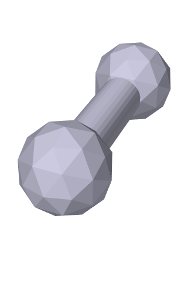
\includegraphics[]{images/dumbbellMesh}&
       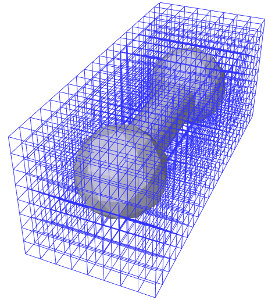
\includegraphics[]{images/dumbbellDistanceGrid}&
       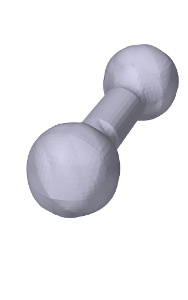
\includegraphics[]{images/dumbbellDistanceSurface}
    \else
       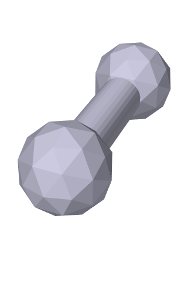
\includegraphics[width=1.75in]{images/dumbbellMesh}&
       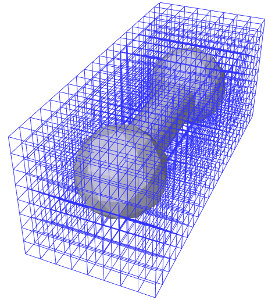
\includegraphics[width=2.5in]{images/dumbbellDistanceGrid}&
       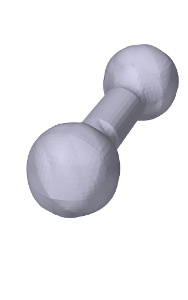
\includegraphics[width=1.75in]{images/dumbbellDistanceSurface}
    \fi
  \end{tabular}
\end{center}
\caption{A mesh used to generate a distance grid, (left), along with a
visualization of the grid itself (middle) and the corresponding
quadratic isosurface (right). Notice how in this case the quadratic
isosurface is smoother than the coarser features of the
original mesh.}
\label{rigidBodySurfacesAndGrid:fig}
\end{figure}

\begin{figure}[ht]
\begin{center}
  \begin{tabular}{cc}
    \iflatexml
       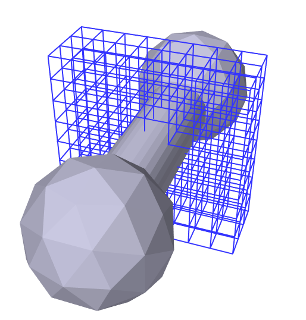
\includegraphics[]{images/dumbbellDistanceGridSub}&
       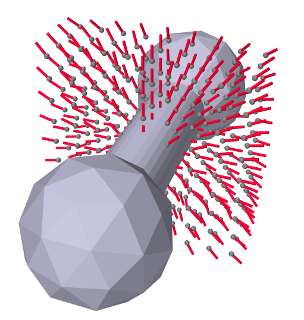
\includegraphics[]{images/dumbbellDistanceGridGrad}
    \else
       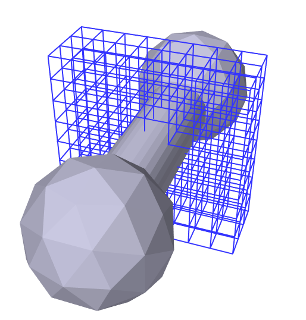
\includegraphics[width=2in]{images/dumbbellDistanceGridSub}&
       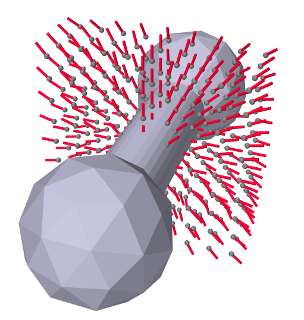
\includegraphics[width=2in]{images/dumbbellDistanceGridGrad}
    \fi
  \end{tabular}
\end{center}
\caption{Rendering a subportion of a distance grid
restricted along the x axis by setting {\sf renderRanges} 
to {\tt "9:12 * *"}, with render properties set to show the grid cells
(left), and the vertices and normals (right).}
\label{rigidBodySubGrid:fig}
\end{figure}

When visualizing the isosurface for a distance grid, it is generally
convenient to also turn {\it off} visualization for the meshes used to
generate the grid. For {\tt RigidBody} objects, this can be
accomplished easily using the convenience property {\sf
gridSurfaceRendering}. If set {\tt true}, it will cause the
isosurface to be rendered {\it instead} of its mesh components.  The
isosurface type will be that indicated by the grid component's {\sf
surfaceType} property, and the rendering will occur independently of
the visibility settings for the meshes or the grid component.

\section{Transforming geometry}
\label{TransformingGeometry:sec}

Certain ArtiSynth components, including {\tt MechModel}, implement the
interface \javaclass[artisynth.core.modelbase]{TransformableGeometry},
which allows the geometric transformation of the component's
attributes (such as meshes, points, frame locations, etc.), along with
its descendant components. The interface provides the method
%
\begin{lstlisting}[]
   public void transformGeometry (AffineTransform3dBase X);
\end{lstlisting}
%
where {\tt X} is an \javaclass[maspack.matrix]{AffineTransform3dBase}
that may be either a \javaclass[maspack.matrix]{RigidTransform3d} or a
more general \javaclass[maspack.matrix]{AffineTransform3d} (Section
\ref{RigidTransform3d:sec}).

\javamethodAlt{artisynth.core.modelbase.TransformableGeometry.transformGeometry()}%
{transformGeometry(X)}
can be used to translate, rotate, shear or scale components. It
can be applied to an entire model or individual components. Unlike
\javamethod*[artisynth.core.util.ScalableUnits]{scaleDistance()}, it
actually changes the physical geometry and so may change the
simulation behavior. For example, applying {\tt transformGeometry()}
to a \javaclass[artisynth.core.mechmodels]{RigidBody} will cause the
shape of its mesh to change, which will change its mass if its {\sf
inertiaMethod} property is set to {\tt DENSITY}.
Figure \ref{RigidAndAffineTransforms:fig} shows a simplified
illustration of both rigid and affine transformations being applied to
a model.

\begin{figure}[ht]
\begin{center}
   \begin{tabular}{ccc}
   \iflatexml
      \includegraphics[width=2truein]{images/tgenModel} &
      \includegraphics[width=2truein]{images/tgenModelRigid} &
      \includegraphics[width=2truein]{images/tgenModelAffine}
   \else
      \includegraphics[width=0.27\textwidth]{images/tgenModel} &
      \includegraphics[width=0.34\textwidth]{images/tgenModelRigid} &
      \includegraphics[width=0.34\textwidth]{images/tgenModelAffine}
   \fi
   \end{tabular}
\end{center}
\caption{Simple illustration of a model (left) undergoing a rigid
transformation (middle) and an affine transformation (right).}
\label{RigidAndAffineTransforms:fig}
\end{figure}

The example below shows how to apply a transformation to a model in
code. In it, a {\tt MechModel} is first scaled by the factors 1.5, 2,
and 3 along the x, y, and z axes, and then flipped upside down using a
{\tt RigidTransform3d} that rotates it by 180 degrees about the x
axis:
%
\begin{lstlisting}[]
   MechModel mech;

   ... build mech model ...

   AffineTransform3d X = new AffineTransform3d();
   X.applyScaling (1.5, 2, 3);
   mech.transformGeometry (X);
   
   RigidTransform3d T = 
      new RigidTransform3d (/*x,y,z=*/0, 0, 0, /*r,p,y=*/0, 0, Math.PI);
   mech.transformGeometry (T);
\end{lstlisting}
%

\subsection{Nonlinear transformations}

The \javaclass[artisynth.core.modelbase]{TransformableGeometry}
interface also supports general, nonlinear geometric transforms.
This can be done using a
\javaclass[maspack.geometry]{GeometryTransformer}, which is an
abstract class for performing general transformations.  To apply such
a transformation to a component, one can create and initialize an appropriate
subclass of {\tt
GeometryTransformer} to perform the desired transformation, and
then apply it using the static {\tt transform} method of the utility class 
\javaclass[artisynth.core.modelbase]{TransformGeometryContext}:
%
\begin{lstlisting}[]
  ModelComponent comp;     // component to be transformed
  GeometryTransformer gtr; // transformer to do the transforming

  ... instantiate and initialize the transformer ...

  TransformGeometryContext.transform (comp, gtr, /*flags=*/0);
\end{lstlisting}
%

At present, the following subclasses of {\tt GeometryTransformer} are
available:

\begin{description}

\item[\protect{\javaclass[maspack.geometry]{RigidTransformer}}]\mbox{}

Implements rigid 3D transformations.

\item[\protect{\javaclass[maspack.geometry]{AffineTransformer}}]\mbox{}

Implements affine 3D transformations.

\item[\protect{\javaclass[artisynth.core.femmodels]{FemGeometryTransformer}}]\mbox{}

Implements a general transformation, using the deformation field
induced by a finite element model. 

\end{description}

\javaclass[artisynth.core.modelbase]{TransformGeometryContext} also
supplies the following convenience methods to apply transformations to
components or collections of components:
%
\begin{lstlisting}[]
    void transform (Iterable<TransformableGeometry>, GeometryTransformer, int);
    void transform (TransformableGeometry[], GeometryTransformer, int);

    void transform (TransformableGeometry, AffineTransform3dBase, int);
    void transform (Iterable<TransformableGeometry>, AffineTransform3dBase, int);
    void transform (TransformableGeometry[], AffineTransform3dBase, int);
\end{lstlisting}
%
The last three of these methods create an instance of either
\javaclass[maspack.geometry]{RigidTransformer} or
\javaclass[maspack.geometry]{AffineTransformer} for the supplied
\javaclass[maspack.matrix]{AffineTransform3dBase}. In fact, most
{\tt TransformableGeometry} components implement their
\javamethodAlt{artisynth.core.modelbase.TransformableGeometry.transformGeometry()}%
{transformGeometry(X)} method as follows:
%
\begin{lstlisting}[]
   public void transformGeometry (AffineTransform3dBase X) {
      TransformGeometryContext.transform (this, X, 0);
   }
\end{lstlisting}
%

The \javaclass[artisynth.core.femmodels]{FemGeometryTransformer}
class is derived from the
class \javaclass[maspack.geometry]{DeformationTransformer}, which uses
the single method
\javaclass[maspack.geometry.DeformationTransformer]{getDeformation()} to
obtain deformation field information at a specified reference position:
%
\begin{lstlisting}[]
    void getDeformation (Vector3d p, Matrix3d F, Vector3d r)
\end{lstlisting}
%
If the deformation field is described by $\x' = f(\x)$, then
for a given reference position $\r$ (in undeformed coordinates),
this method should return the deformed position $\p = f(\r)$
and the deformation gradient
%
\begin{equation}
\F \equiv \frac{\partial f}{\partial \x}
\end{equation}
%
evaluated at $\r$. 

\javaclass[artisynth.core.femmodels]{FemGeometryTransformer} obtains
$f(\x)$ and $\F$ from a
\javaclass[artisynth.core.femmodels]{FemModel3d} (see Section
\ref{FEMModels:sec}) whose elemental rest positions enclose the
components to be transformed, using the fact that a finite element
model creates an implied piecewise-smooth deformation field as it
deviates from its rest position. For each reference point $\r$ needed
by the transformation process, {\tt FemGeometryTransformer} finds the
FEM element whose rest volume encloses $\r$, and then uses the
corresponding shape function coordinates to compute $f(\x)$ and $\F$
from the element's deformation. If the FEM model does {\it not}
enclose $\r$, the nearest element is used to determine the shape
function coordinates (however, this calculation becomes less accurate and
meaningful the farther $\r$ is from the FEM model). Transformations based
on FEM models are further illustrated in Section
\ref{FemModelDeformer:sec}, and by Figure
\ref{JointedCollideDeformation:fig}. Full details on ArtiSynth finite
element models are given in Section \ref{FEMModels:sec}.

Besides FEM models, there are numerous other ways to create
deformation fields, such as radial basis functions, thin plate
splines, etc. Some of these may be more appropriate for a particular
application and can provide deformations that are globally smooth (as
opposed to piecewise smooth).  It should be relatively easy for an
application to create its own subclass of {\tt DeformationTransformer}
to implement the deformation of choice by overriding the single
\javaclass[maspack.geometry.DeformationTransformer]{getDeformation()}
method.

\subsection{Example: the FemModelDeformer class}
\label{FemModelDeformer:sec}

An FEM-based geometric transformation of a {\tt MechModel} is
facilitated by the class
\javaclass[artisynth.core.workspace]{FemModelDeformer}, which one can
add to an existing {\tt RootModel} to transform the geometry of a {\tt
MechModel} already located within that {\tt RootModel}.  {\tt
FemModelDeformer} subclasses
\javaclass[artisynth.core.femmodels]{FemModel3d} to include a
\javaclass[artisynth.core.femmodels]{FemGeometryTransformer}, and
provides some utility methods to support the transformation process.

A {\tt FemModelDeformer} can be added to a {\tt RootModel} by adding
the following code fragment to the end of the {\tt build()} method:
%
\begin{lstlisting}[]
   public void build (String[] args) {

      ... build the model ...

      FemModelDeformer deformer =
         new FemModelDeformer ("deformer", this, /*maxn=*/10);
      addModel (deformer);
      // add a control panel (this is optional)
      addControlPanel (deformer.createControlPanel());  
   }
\end{lstlisting}
%
When the deformer is created, its constructor searches the specified
{\tt RootModel} to locate the first top-level {\tt MechModel}. It then
creates a hexahedral FEM grid around this model, with {\tt maxn} specifying
the number of cells along the maximum dimension. Material and
mass properties of the model are computed automatically from the
underlying {\tt MechModel} dimensions (but can be altered if necessary after
construction). When added to the {\tt RootModel},
the deformer becomes another top-level model that can be deformed
independently of the {\tt MechModel} to create the required
deformation field, as described below. It also supplies application-defined
menu items that appear under the {\sf Application} menu in the ArtiSynth
menu bar (see Section \ref{MenuItems:sec}). 
The deformer's {\tt createControlPanel()} can also be used
to create a {\tt ControlPanel} (Section \ref{ControlPanels:sec}) that
controls the visibility of the FEM model and the dynamic behavior of
both it and the {\tt MechModel}.

An example is defined in 
%
\begin{verbatim}
  artisynth.demos.tutorial.DeformedJointedCollide
\end{verbatim}
%
where the {\tt JointedCollide} example of Section
\ref{JointedCollide:sec} is extended to include a 
{\tt FemModelDeformer} using the code described above.

\begin{figure}[ht]
\begin{center}
\iflatexml
 \includegraphics[]{images/DeformedJointedCollide}
\else
 \includegraphics[width=5in]{images/DeformedJointedCollide}
\fi
\end{center}
\caption{The {\tt DeformedJointedCollide} example initially loaded
into ArtiSynth.}
\label{DeformedJointedCollide:fig}
\end{figure}

To load this example in ArtiSynth, select {\sf All demos > tutorial >
DeformedJointedCollide} from the {\sf Models} menu. The model should load and
initially appear as in Figure \ref{DeformedJointedCollide:fig}, where
the control panel appears on the right.

The underlying {\tt MechModel} (or "model") can now be
transformed by first deforming the FEM model (or "grid") and
then using the resulting deformation field to effect the
transformation:

\begin{enumerate}

\item Make the model non-dynamic and the grid dynamic by unchecking
{\sf model dynamic} and checking {\sf grid dynamic} in the control
panel. This means that when simulation is run, the model will be inert
while the grid will respond physically.

\item Deform the grid using simulation. One easy way to do this is to
fix certain nodes, generally on or near the grid boundary, and then
move some of these using the translation or transrotator
tool while simulation is running. To fix a set of nodes, select
them in the viewer, choose {\sf Edit properties ...} from the
right-click context menu, and then uncheck their {\sf dynamic} property.
To easily select a large number of nodes without also selecting
model components or grid elements, one can specify {\tt FemNode}
in the selection filter widget. (See the sections
``Manipulation Tools'' and ``Selection filtering'' in the
\artisynthManual{uiguide}{ArtiSynth User Interface Guide}.)

\item After the grid has been deformed, choose {\sf deform} from the
{\sf Application} menu in the ArtiSynth toolbar to transform the model.
Afterwards, the transformation can be undone by choosing {\sf undo},
and the grid can be reset by choosing {\sf reset grid}.

\item To run the deformed model after the transformation, it should
again be made dynamic by checking {\sf model dynamic} in the control
panel.  The itself grid can be made non-dynamic, and it and/or its
nodes can be made invisible by unchecking {\sf grid visible} and/or
{\sf grid nodes visible} in the control panel.

\end{enumerate}

The result of a possible deformation is shown in Figure
\ref{JointedCollideDeformation:fig}.

\begin{figure}[ht]
\begin{center}
  \begin{tabular}{cc}
  \iflatexml
    \includegraphics[]{images/DeformedJointedCollideBefore}&
    \includegraphics[]{images/DeformedJointedCollideAfter}
  \else
    \includegraphics[width=0.45\textwidth]{images/DeformedJointedCollideBefore}&
    \includegraphics[width=0.45\textwidth]{images/DeformedJointedCollideAfter}
  \fi
  \end{tabular}
\end{center}
\caption{Deformation achieved in {\tt DeformedJointedCollide},
showing both the model and grid (using an orthographic view)
before and after the deformation.}
\label{JointedCollideDeformation:fig}
\end{figure}

\begin{sideblock}
Note: {\tt FemModelDeformer} is not intended to provide a general
purpose solution to nonlinear geometric transformations. Rather, it
is mainly intended to illustrate the capabilities of
\javaclass[maspack.geometry]{GeometryTransformer} and the
\javaclass[artisynth.core.modelbase]{TransformableGeometry} interface.
\end{sideblock}

\subsection{Implementation and behavior}

As indicated above, the management of transforming the geometry for one
or more components is handled by the
\javaclass[artisynth.core.modelbase]{TransformGeometryContext} class.
The transform operations themselves are carried out by this class's
\javamethod[artisynth.core.modelbase.TransformGeometryContext]{apply()} 
method, which (a) assembles all the components that need
to be transformed, (b) performs the actual transform operations,
(c) invokes any required updating actions on other components,
and finally (d) notifies parent components of the change using
a \javaclass[artisynth.core.modelbase]{GeometryChangeEvent}.

To support this, ArtiSynth components which implement
\javaclass[artisynth.core.modelbase]{TransformableGeometry}
must also supply the methods
%
\begin{lstlisting}[]
   public void addTransformableDependencies (
      TransformGeometryContext context, int flags);

   public void transformGeometry (
      GeometryTransformer gtr, TransformGeometryContext context, int flags);
\end{lstlisting}
%
The first method,
\javamethodAlt{%
artisynth.core.modelbase.TransformableGeometry.addTransformableDependencies()}%
{addTransformableDependencies(context,flags)}, 
is called in step (a) to add to the context any additional components
which should be transformed along with this component. This includes
any descendants which should be transformed, since the
transformation of these should not generally be done within {\tt
transformGeometry(gtr,context,flags)}.

The second method, 
\javamethodAlt{%
artisynth.core.modelbase.TransformableGeometry.transformGeometry(,,)}%
{transformGeometry(gtr,context,flags)}, is
called in step (b) to perform the actual transformation on this
component.  It should use the supplied geometry transformer {\tt gtr}
to transform its attributes, as well as {\tt context} to query what
other components are also being transformed and to request
any needed updating actions to be called in step (c).  The {\tt flags} argument
specifies conditions associated with the transformation, which at the
moment may currently include:

\begin{description}

\item[TG\_SIMULATING]\mbox{}

The system is currently simulating, and therefore it may not be
desirable to transform all attributes;

\item[TG\_ARTICULATED]\mbox{}

Rigid body articulation constraints should
be enforced as the transform proceeds.

\end{description}

Full details for all this are given in the documentation for
\javaclass[artisynth.core.modelbase]{TransformGeometryContext}.

The transforming behavior of a component is up to its implementing
method, but the following rules are generally observed:

\begin{enumerate}

\item Transformable descendants are also transformed, by using {\tt
addTransformableDependencies()} to add them to the context as described
above;

\item When the nodes of an FEM model (Section \ref{FEMModels:sec}) are
transformed, the rest positions are also transformed if the system is
not simulating (i.e., if the {\tt TG\_SIMULATING} flag is not set).
This also causes the mass of the adjacent nodes to be recomputed from
the densities of the adjacent elements;

\item When dynamic components are transformed, any attachments and
constraints associated with them are updated appropriately, but only
if the system is not simulating. Non-transforming dynamic components
that are attached to transforming components as slaves are generally
updated so as to follow the transforming components to which they are
attached.

\end{enumerate}

\subsection{Use in model registration}

Transforming model geometry can obviously be used as part of the
process of creating subject-specific biomechanical and anatomical
models. However, registration will generally require more that
geometric transformation, since other properties, such as material
stiffnesses, densities, and maximum forces will generally need to be
adjusted as well. As a specific example, when applying a geometric
transform to a model containing {\tt AxialSprings}, the {\tt
restLength} properties of the springs will be unchanged, whereas the
initial lengths may be, resulting in a different applied forces and
physical behavior.

\section{General component arrangements}

As discussed in Section \ref{MechModel:sec} and elsewhere, a {\tt
MechModel} provides a number of predefined child components for
storing particles, rigid bodies, springs, constraints, and other
components.  However, applications are not required to store their
components in these containers, and may instead create any sort of
component arrangement desired.

For example, suppose that one wishes to create a biomechanical model
of both the right and left human arms, consisting of bones,
point-to-point muscles, and joints. The standard containers supplied
by \javaclass[artisynth.core.mechmodels]{MechModel} would require that
all the components be placed within the following containers:
%
\begin{lstlisting}[]
   rigidBodies          // all bones
   axialSprings         // all point-to-point muscles
   connectors           // all joints
\end{lstlisting}
%
Instead of this, one may wish to set up a more appropriate component
hierarchy, such as
%
\begin{lstlisting}[]
   leftArm              // left-arm components
      bones             //   left bones
      muscles           //   left muscles
      joints            //   left joints
   rightArm             // right-arm components
      bones             //   right bones
      muscles           //   right muscles
      joints            //   right joints
\end{lstlisting}
%
To do this, the application {\tt build()} method can create the
necessary hierarchy and then
populate it with whatever components are desired.  Before simulation
begins (or whenever the model structure is changed), the {\tt
MechModel} will recursively traverse the component hierarchy and
update whatever internal structures are needed to run the
simulation.

\subsection{Container components}

The generic class \javaclass[artisynth.core.modelbase]{ComponentList}
can be used as a container for model components of a specific type.
It can be created using a declaration of the form
%
\begin{lstlisting}[]
   ComponentList<Particle> list = new ComponentList<Type> (Type.class, name);
\end{lstlisting}
%
where {\tt Type} is the class type of the components and {\tt name} is
the name for the container. Once the container is created, it should
be added to the {\tt MechModel} (or another internal container) and 
populated with child components of the specified type.
For example,
\begin{lstlisting}[]
   MechModel mech; 
   ...
   ComponentList<Particle> parts = 
      new ComponentList<Particle> (Particle.class, "parts");
   ComponentList<Frame> frames = 
      new ComponentList<Frame> (Frame.class, "frames");

   // add containers to the mech model
   mech.add (parts); 
   mech.add (frames);
\end{lstlisting}
creates two containers named {\tt "parts"} and {\tt "frames"} for
storing components of type {\tt Particle} and {\tt Frame},
respectively, and adds them to a {\tt MechModel} referenced by {\tt
mech}.

In addition to {\tt ComponentList}, applications may use several
"specialty" container types which are subclasses of {\tt
ComponentList}:

\begin{description}

\item[RenderableComponentList]\mbox{}

A subclass of {\tt ComponentList}, that
has its {\it own} set of render properties which can be inherited by
its children. This can be useful for compartmentalizing render
behavior.  Note that it is {\it not} necessary to store renderable
components in a {\tt RenderableComponentList}; components stored in a
{\tt ComponentList} will be rendered too.

\item[PointList]\mbox{}

A {\tt RenderableComponentList} that is optimized for
rendering points, and also contains its own {\tt pointDamping}
property that can be inherited by its children.

\item[PointSpringList]\mbox{}

A {\tt RenderableComponentList} designed for
storing point-based springs. It contains a {\tt material} property that
specifies a default axial material that can be used by its children.

\item[AxialSpringList]\mbox{}

A {\tt PointSpringList} that is optimized for
rendering two-point axial springs.

\end{description}

If necessary, it is relatively easy to define one's own customized
list by subclassing one of the other list types. One of the main
reasons for doing so, as suggested above, is to supply default
properties to be inherited by the list's descendants.  

A component list which declares {\tt ModelComponent} as its type can
be used to store {\tt any} type of component, including other
component lists. This allows the creation of arbitrary component
hierarchies. Generally either\\
{\tt ComponentList<ModelComponent>} or 
{\tt RenderableComponentList<ModelComponent>} are
best suited to implement hierarchical groupings.

\subsection{Example: a net formed from balls and springs}

\begin{figure}[ht]
\begin{center}
\iflatexml
 \includegraphics[]{images/NetDemo}
\else
 \includegraphics[width=3.75in]{images/NetDemo}
\fi
\end{center}
\caption{NetDemo model loaded into ArtiSynth.}
\label{NetDemo:fig}
\end{figure}

A simple example showing an arrangement of balls and springs formed into
a net is defined in
%
\begin{verbatim}
  artisynth.demos.tutorial.NetDemo
\end{verbatim}
%

The {\tt build()} method and some of the supporting definitions for
this example are shown below.
%
\lstset{numbers=left}
\begin{lstlisting}[]
   protected double stiffness = 1000.0;   // spring stiffness
   protected double damping = 10.0;       // spring damping
   protected double maxForce = 5000.0;    // max force with excitation = 1
   protected double mass = 1.0;           // mass of each ball
   protected double widthx = 20.0;        // width of the net along x
   protected double widthy = 20.0;        // width of the net along y
   protected int numx = 8;                // num balls along x
   protected int numy = 8;                // num balls along y

   // custom component containers
   protected MechModel mech;
   protected PointList<Particle> balls;
   protected ComponentList<ModelComponent> springs;   
   protected RenderableComponentList<AxialSpring> greenSprings;
   protected RenderableComponentList<AxialSpring> blueSprings;

   private AxialSpring createSpring (
      PointList<Particle> parts, int idx0, int idx1) {
      // create a "muscle" spring connecting particles indexed by 'idx0' and
      // 'idx1' in the list 'parts'
      Muscle spr = new Muscle (parts.get(idx0), parts.get(idx1));
      spr.setMaterial (new SimpleAxialMuscle (stiffness, damping, maxForce));
      return spr;
   }

   public void build (String[] args) {

      // create MechModel and add to RootModel
      mech = new MechModel ("mech");
      mech.setGravity (0, 0, -980.0);
      mech.setPointDamping (1.0);
      addModel (mech);

      int nump = (numx+1)*(numy+1); // nump = total number of balls

      // create custom containers:
      balls = new PointList<Particle> (Particle.class, "balls");
      springs = new ComponentList<ModelComponent>(ModelComponent.class,"springs");
      greenSprings = new RenderableComponentList<AxialSpring> (
         AxialSpring.class, "greenSprings");
      blueSprings = new RenderableComponentList<AxialSpring> (
         AxialSpring.class, "blueSprings");

      // create balls in a grid pattern and add to the list 'balls'
      for (int i=0; i<=numx; i++) {
         for (int j=0; j<=numy; j++) {
            double x = widthx*(-0.5+i/(double)numx);
            double y = widthy*(-0.5+j/(double)numy);
            Particle p = new Particle (mass, x, y, /*z=*/0);
            balls.add (p);
            // fix balls along the edges parallel to y
            if (i == 0 || i == numx) {
               p.setDynamic (false);
            }
         }
      }

      // connect balls by green springs parallel to y
      for (int i=0; i<=numx; i++) {
         for (int j=0; j<numy; j++) {
            greenSprings.add (
               createSpring (balls, i*(numy+1)+j, i*(numy+1)+j+1));
         }
      }
      // connect balls by blue springs parallel to x
      for (int j=0; j<=numy; j++) {
         for (int i=0; i<numx; i++) {
            blueSprings.add (
               createSpring (balls, i*(numy+1)+j, (i+1)*(numy+1)+j));
         }
      }

      // add containers to the mechModel
      springs.add (greenSprings);
      springs.add (blueSprings);
      mech.add (balls);
      mech.add (springs);

      // set render properties for the components      
      RenderProps.setLineColor (greenSprings, new Color(0f, 0.5f, 0f));
      RenderProps.setLineColor (blueSprings, Color.BLUE);
      RenderProps.setSphericalPoints (mech, widthx/50.0, Color.RED);
      RenderProps.setCylindricalLines (mech, widthx/100.0, Color.BLUE);
   }
\end{lstlisting}
\lstset{numbers=none}
%
The {\tt build()} method begins by creating a {\tt MechModel} in the
usual way (lines 29-30). It then creates a net composed of a set of
balls arranged as a uniform grid in the x-y plane, connected by a set
of green colored springs running parallel to the y axis and a set of
blue colored springs running parallel to the x axis. These are
arranged into a component hierarchy of the form
%
\begin{lstlisting}[]
   balls
   springs
      greenSprings
      blueSprings
\end{lstlisting}
%
using containers created at lines 37-42. The balls are then created
and added to {\tt balls} (lines 45-56), the springs are created and
added to {\tt greenSprings} and {\tt blueSprings} (lines 59-71), and
the containers are added to the {\tt MechModel} at lines 74-77.
The balls along the edges parallel to the y axis are fixed.
Render properties are set at lines 80-83, with the colors for {\tt
greenSprings} and {\tt blueSprings} being explicitly set to dark green
and blue.

\begin{sideblock}
{\tt MechModel}, along with other classes derived from {\tt
ModelBase}, enforces {\it reference containment}. That means that all
components referenced by components within a {\tt MechModel} must
themselves be contained within the {\tt MechModel}.  This condition is
checked whenever a component is added directly to a {\tt MechModel} or
one of its ancestors. This means that the components must be added to
the {\tt MechModel} in an order that ensures any referenced components are
already present. For example, in the {\tt NetDemo} example above, adding the
particle list {\it after} the spring list would generate an error.
\end{sideblock}

To run this example in ArtiSynth, select {\sf All demos > tutorial >
NetDemo} from the {\sf Models} menu. The model should load and
initially appear as in Figure \ref{NetDemo:fig}.  Running the model
will cause the net to fall and sway under gravity. When the ArtiSynth
navigation panel is opened and expanded, the component hierarchy will
appear as in Figure \ref{NetDemoNav:fig}. While the standard
{\tt MechModel} containers are still present, they are not displayed
by default because they are empty.

\begin{figure}[ht]
\begin{center}
\iflatexml
 \includegraphics[]{images/NetDemoNav}
\else
 \includegraphics[width=2.25in]{images/NetDemoNav}
\fi
\end{center}
\caption{NetDemo components displayed in the ArtiSynth navigation panel.}
\label{NetDemoNav:fig}
\end{figure}

\subsection{Adding containers to other models}

In addition to {\tt MechModel}, application-defined containers can be
added to any model that inherits from
\javaclass[artisynth.core.modelbase]{ModelBase}. This includes {\tt
RootModel} and {\tt FemModel}. However, at the present time,
components added to such containers won't do anything, other than be
rendered in the viewer if they are
\javaclass[maspack.render]{Renderable}.

